\chapter{Register Machines}

\begin{sidenotebox}{Register Machine Simulator}
	\begin{center}
		\begin{tabular}{c c}
			\href{https://flutter-rm.herokuapp.com/#/}{Register Machine Simulator} &  \href{https://github.com/MMZK1526/Haskell-RM}{Repository} \\
		\end{tabular}
	\end{center}
	This simulator has been developed by Yìtáng Chén to support 50003, make sure to give him a $\bigstar$! 
\end{sidenotebox}
\section{Algorithms}

\begin{definitionbox}{Hilbert's Entscheidungsproblem (Decision Problem)}
	A problem proposed by David Hilbert and Wilhem Ackermann in 1928. Considering if there is an algorithm to determine if any statement is universally valid (valid in every structure satisfying the axioms - facts within the logic system assumed to be true (e.g in maths $1 + 0 = 1$)).
	\\
	\\ This can be also be expressed as an algorithm that can determine if any first-order logic statement is provable given some axioms.
	\\
	\\ It was proven that no such algorithm exists by Alonzo Church and Alan Turing using their notions of Computing which show it is not computable.
\end{definitionbox}

\begin{definitionbox}{Algorithms Informally}
	One definition is: \textit{A finite, ordered series of steps to solve a problem.}
	\\
	\\ Common features of the many definitions of algorithms are:
    \begin{center}
        \begin{tabular}{l p{.8\textwidth}}
            \textbf{Finite} & Finite number of elementary (cannot be broken down further) operations. \\
            \textbf{Deterministic} & Next step uniquely defined by the current. \\
            \textbf{Terminating}? & May not terminate, but we can see when it does \& what the result is. \\
        \end{tabular}
    \end{center}
    \begin{center}
        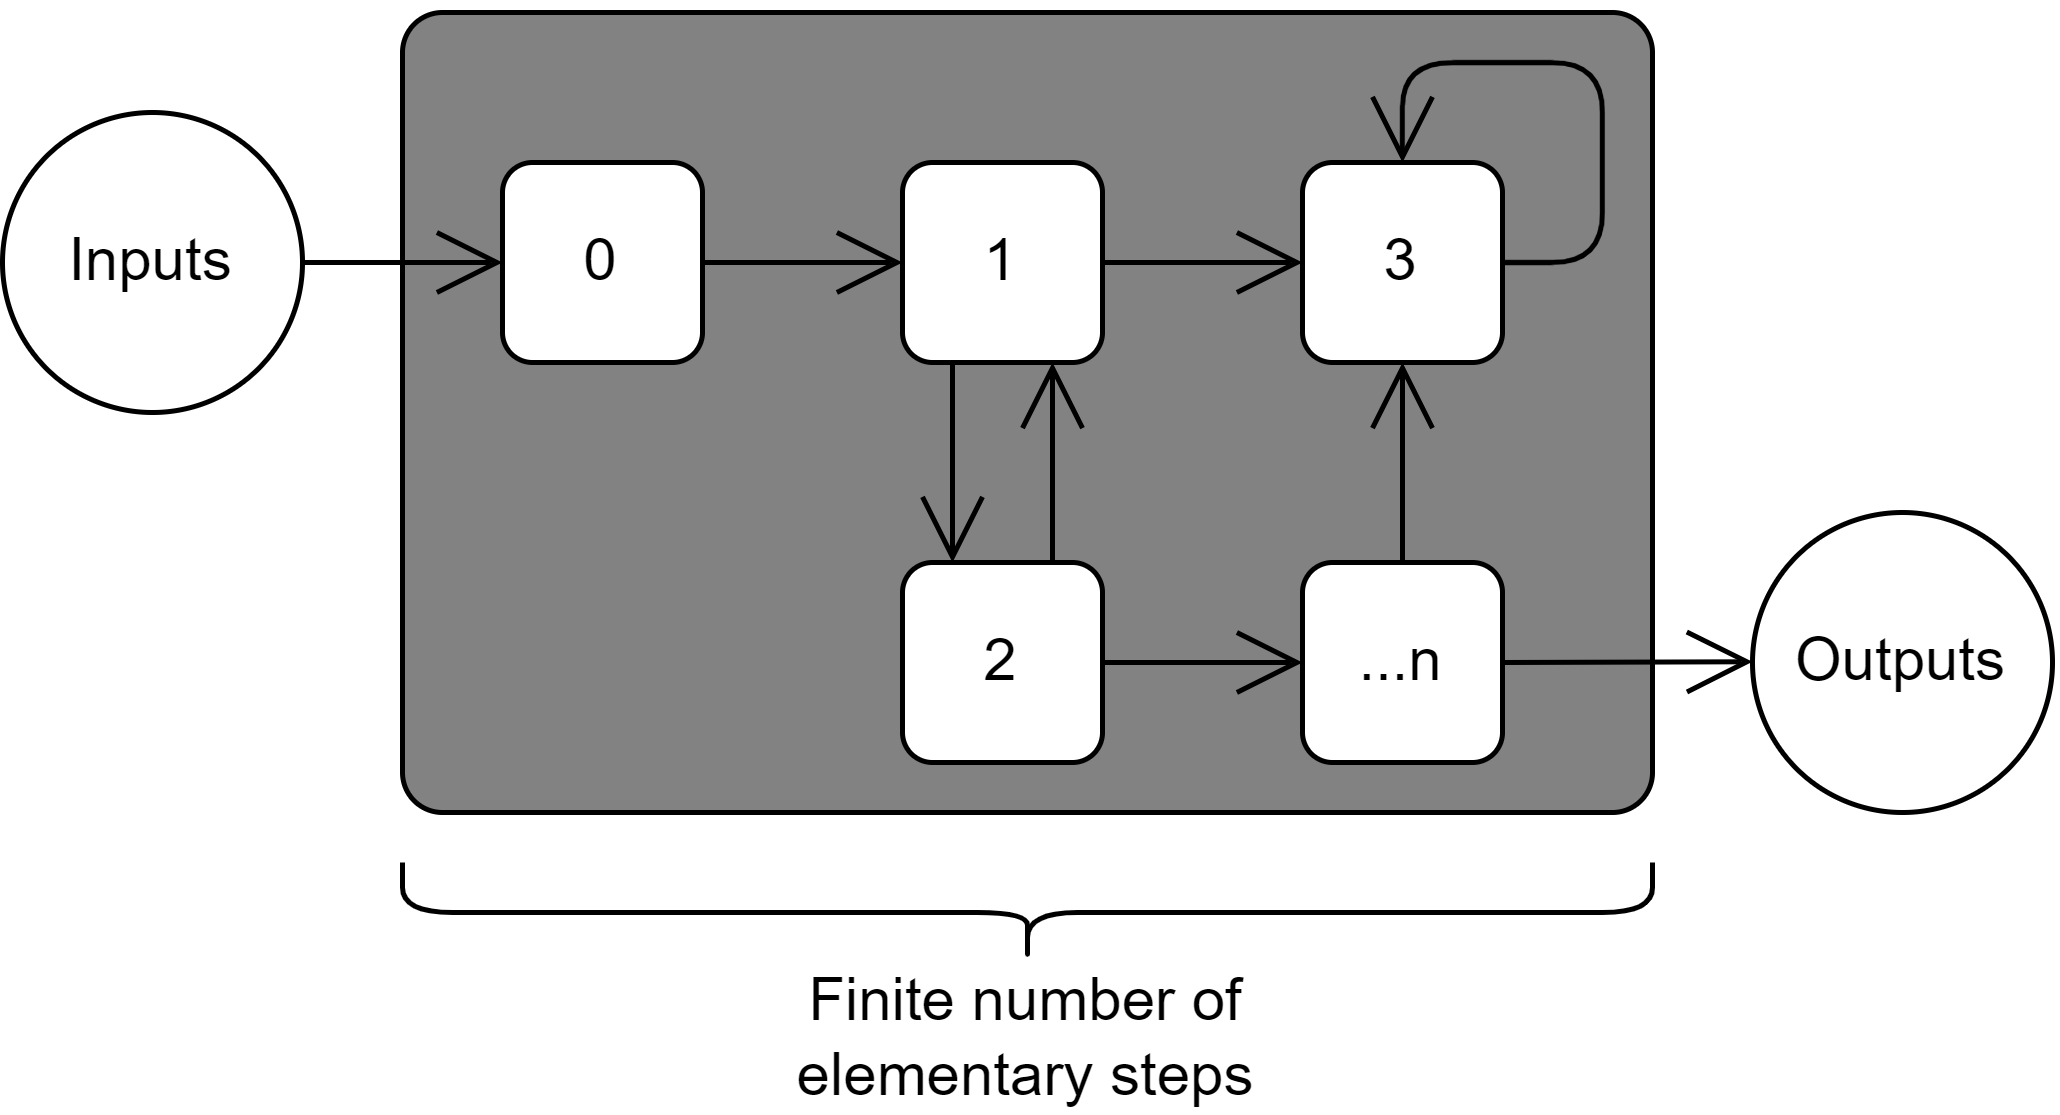
\includegraphics[width=0.6\textwidth]{register_machines/images/algorithm.drawio.png}
    \end{center}
\end{definitionbox}

\section{Register Machines}

\begin{definitionbox}{Register Machine}
	A turing-equivalent (same computational power as a turing machine) abstract machine that models what is computable.
	\begin{itemize}
		\item Infinitely many registers, each storing a natural number ($\mathbb{N} \triangleq \{0, 1, 2, \dots\}$)
		\item Each instruction has a label associated with it.
    \end{itemize}
    There are 3 instructions:
    \begin{center}
        \begin{tabular}{l l}
            $\inc{i}{m}$    & Add 1 to register $\reglabel{i}$ and then jump to the instruction at $\instrlabel{m}$               \\
            $\dec{i}{n}{m}$ & If $\reglabel{i} > 0$ then decrement it and jump to $\instrlabel{n}$, else jump to $\instrlabel{m}$ \\
            $\halt$         & Halt the program.
        \end{tabular}
    \end{center}
	At each point in a program the registers are in a configuration $c = (l, r_0, \dots, r_n)$ (where $r_i$ is the value of $\reglabel{i}$ and $l$ is the instruction label $\instrlabel{l}$ that is about to be run).
	\begin{itemize}
		\item $c_0$ is the initial configuration, next configurations are $c_1, c_2, \dots$.
		\item In a finite computation, the final configuration is the \textbf{halting configuration}.
		\item In a \textbf{proper halt} the program ends on a $\halt$.
		\item In an \textbf{erroneous halt} the program jumps to a non-existent instruction, the \textbf{halting configuration} is for the instruction immediately before this jump.
    \end{itemize}
    \begin{center}
        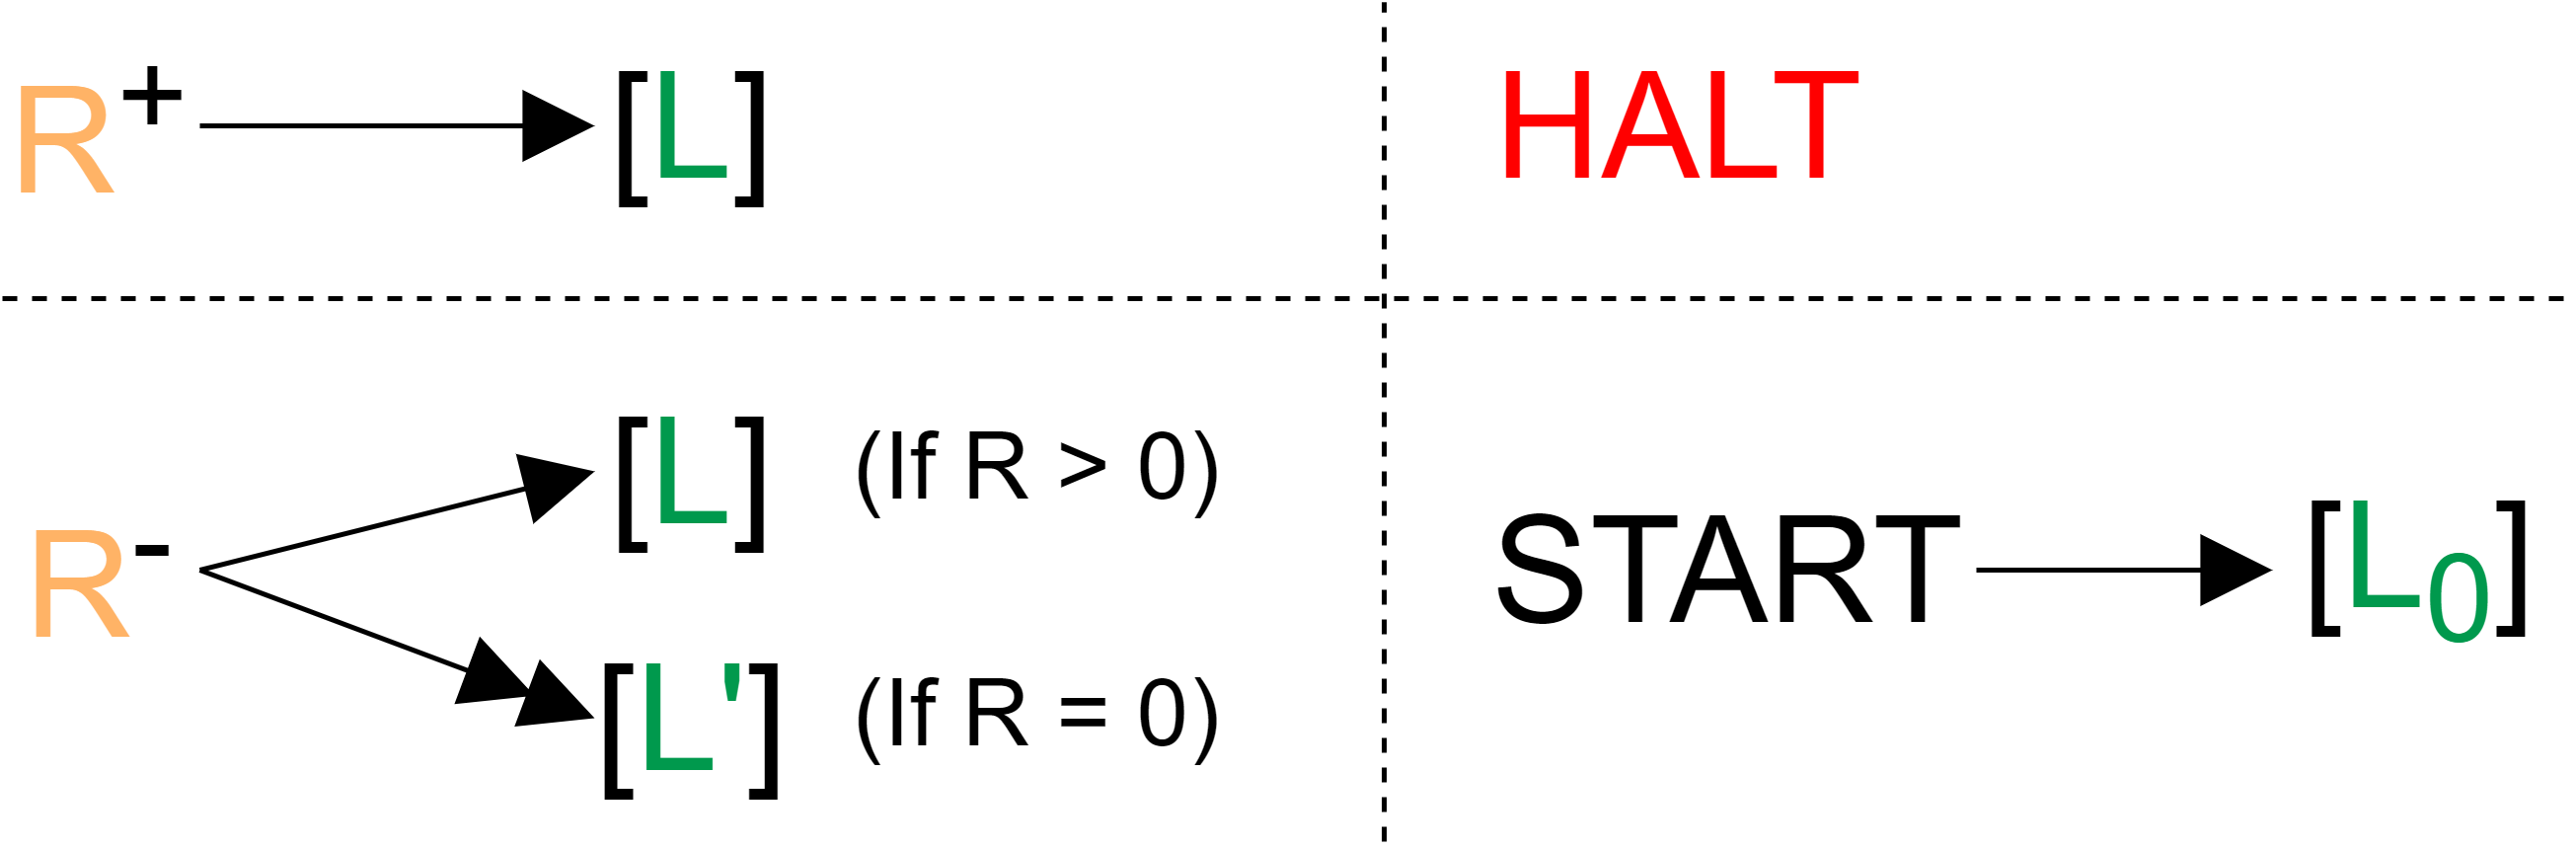
\includegraphics[width=0.6\textwidth]{register_machines/images/graphical_register_machine.drawio.png}
    \end{center}
\end{definitionbox}

\begin{examplebox}{Sum of three numbers}
	The following register machine computes:
	\[\begin{matrix}
			\reglabel{0} = \reglabel{0} + \reglabel{1} + \reglabel{2} & \reglabel{1} = 0 & \reglabel{2} = 0 \\
		\end{matrix}\]
	Or as a partial function:
	\[f(x,y,z) = x + y + z\]
	\begin{minipage}{0.3\textwidth}
		\subsubsection*{Registers}
		$\begin{matrix}
				\reglabel{0} & \reglabel{1} & \reglabel{2} \\
			\end{matrix}$
		\subsubsection*{Program}
		$\begin{matrix*}[l]
				\instr{0}{\dec{1}{1}{2}}
				\instr{1}{\inc{0}{0}}
				\instr{2}{\dec{2}{3}{4}}
				\instr{3}{\inc{0}{2}}
				\instr{4}{\halt}
			\end{matrix*}$
	\end{minipage}
	\hfill
	\begin{minipage}{0.2\textwidth}
		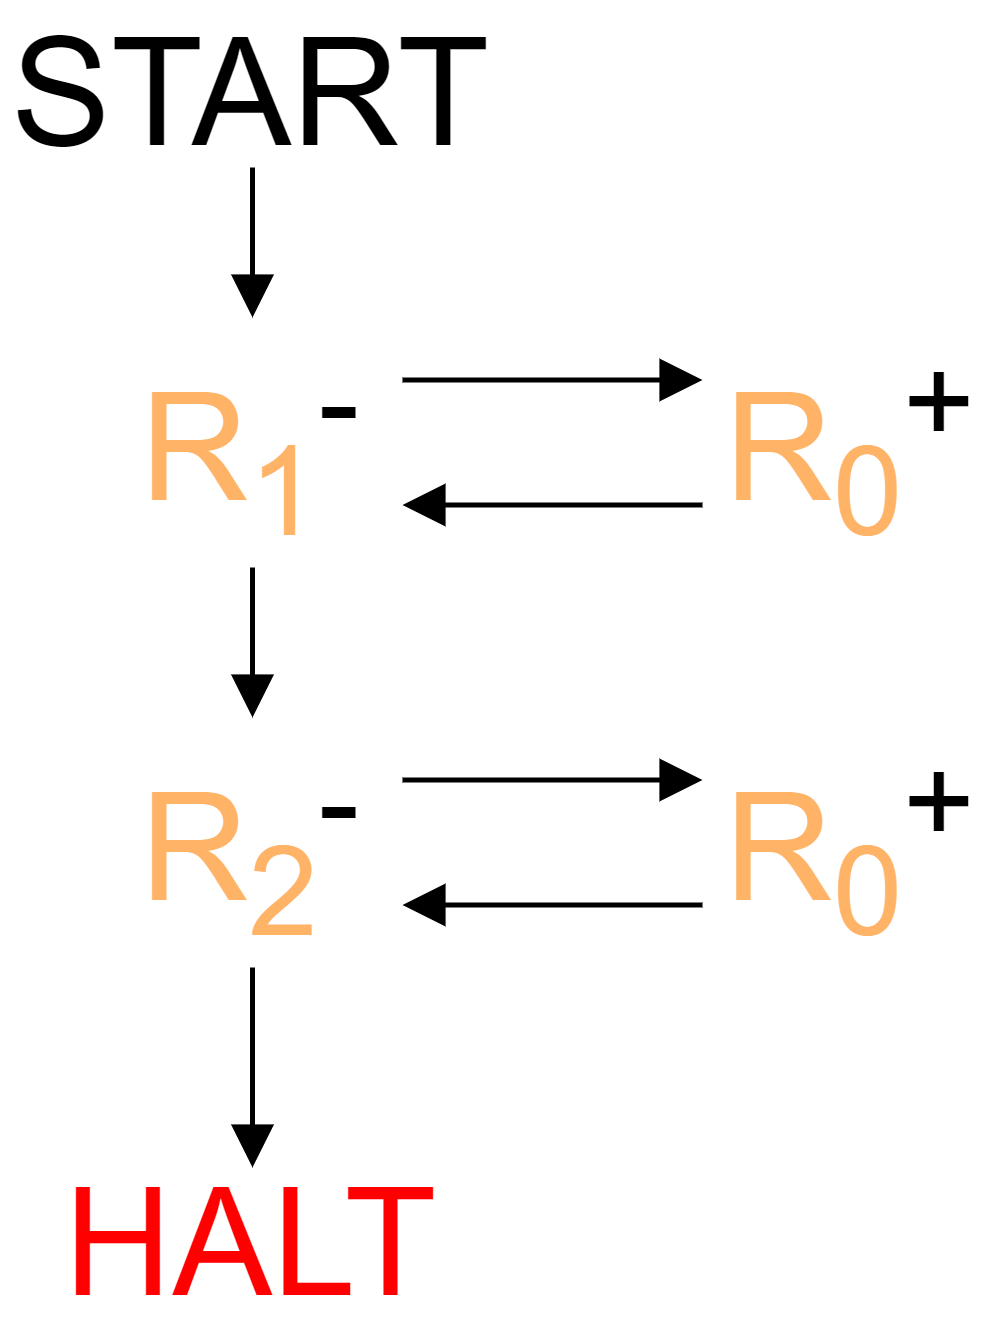
\includegraphics[width=\textwidth]{register_machines/images/graphical_rm_example.drawio.png}
	\end{minipage}
	\hfill
	\begin{minipage}{0.3\textwidth}
		\subsubsection*{Example Configuration}
		\begin{tabular}{l l l l}
			\regconfig{$\instrlabel{i}$}{$\reglabel{0}$}{$\reglabel{1}$}{$\reglabel{2}$}
			\hline
			\regconfig{0}{1}{2}{3}
			\regconfig{1}{1}{1}{3}
			\regconfig{0}{2}{1}{3}
			\regconfig{1}{2}{0}{3}
			\regconfig{0}{3}{0}{3}
			\regconfig{2}{3}{0}{3}
			\regconfig{3}{3}{0}{2}
			\regconfig{2}{4}{0}{2}
			\regconfig{3}{4}{0}{1}
			\regconfig{2}{5}{0}{1}
			\regconfig{3}{5}{0}{0}
			\regconfig{2}{6}{0}{0}
			\regconfig{4}{6}{0}{0}
		\end{tabular}
	\end{minipage}
\end{examplebox}

\subsection{Partial Functions}
\begin{definitionbox}{Partial Function}
	Maps some members of the domain $X$, with each mapped member going to at most one member of the codomain $Y$.
	\[f \subseteq X \times Y \ \text{  and  } \ (x,y_1) \in f \land (x, y_2) \in f \Rightarrow y_1 = y_2\]
	\begin{center}
		\begin{tabular}{l | l}
			$f(x) = y$            & $(x,y) \in f$                                           \\
			$f(x)\downarrow$      & $\exists y \in Y . [f(x) = y]$                          \\
			$f(x)\uparrow$        & $\neg\exists y \in Y . [f(x) = y]$                      \\
			$X \rightharpoonup Y$ & Set of all \textit{partial functions} from $X$ to $Y$. \\
			$X \to Y$             & Set of all \textit{total functions} from $X$ to $Y$.   \\
		\end{tabular}
	\end{center}
	A partial function from $X$ to $Y$ is total if it satisfies $f(x)\downarrow$.
\end{definitionbox}
Register machines can be considered as partial functions as for a given input/initial configuration, they produce at most one halting configuration (as they are deterministic, for non-finite computations/non-halting there is no halting configuration).
\\
\\ We can consider a register machine as a partial function of the input configuration, to the value of the first register in the halting configuration.
\[f \in \mathbb{N}^n \rightharpoonup \mathbb{N} \ \text{  and  } \ (r_0, \dots, r_n) \in \mathbb{N}^n, r_0 \in \mathbb{N}\]
\textit{Note: Many different register machines may compute the same partial function.}

\subsection{Computable Functions}
The following arithmetic functions are computable. Using them we can derive larger register machines for more complex arithmetic (e.g logarithms making use of repeated division).
\subsubsection{Projection}
\trisplit{
	\[p(x,y) \triangleq x\]
	\[(r_0, r_1) \to r_0\]
}{
	\[\halt\]
}{
    \begin{center}
        
\includegraphics[scale=0.06]{register_machines/images/rm_functions/projection.drawio.png}
    \end{center}
}

\subsubsection*{Constant}
\trisplit{
	\[c(x) \triangleq n\]
	\[(r_0) \to n\]
}{
	\[
		\begin{matrix*}[l]
			\instr{0}{\dec{0}{0}{1}}
			\instr{1}{\inc{0}{2}}
			\vdots & \vdots \\
			\instr{n}{\inc{0}{n+1}}
			\instr{n+1}{\halt}
		\end{matrix*}
	\]
}{
    \begin{center}
        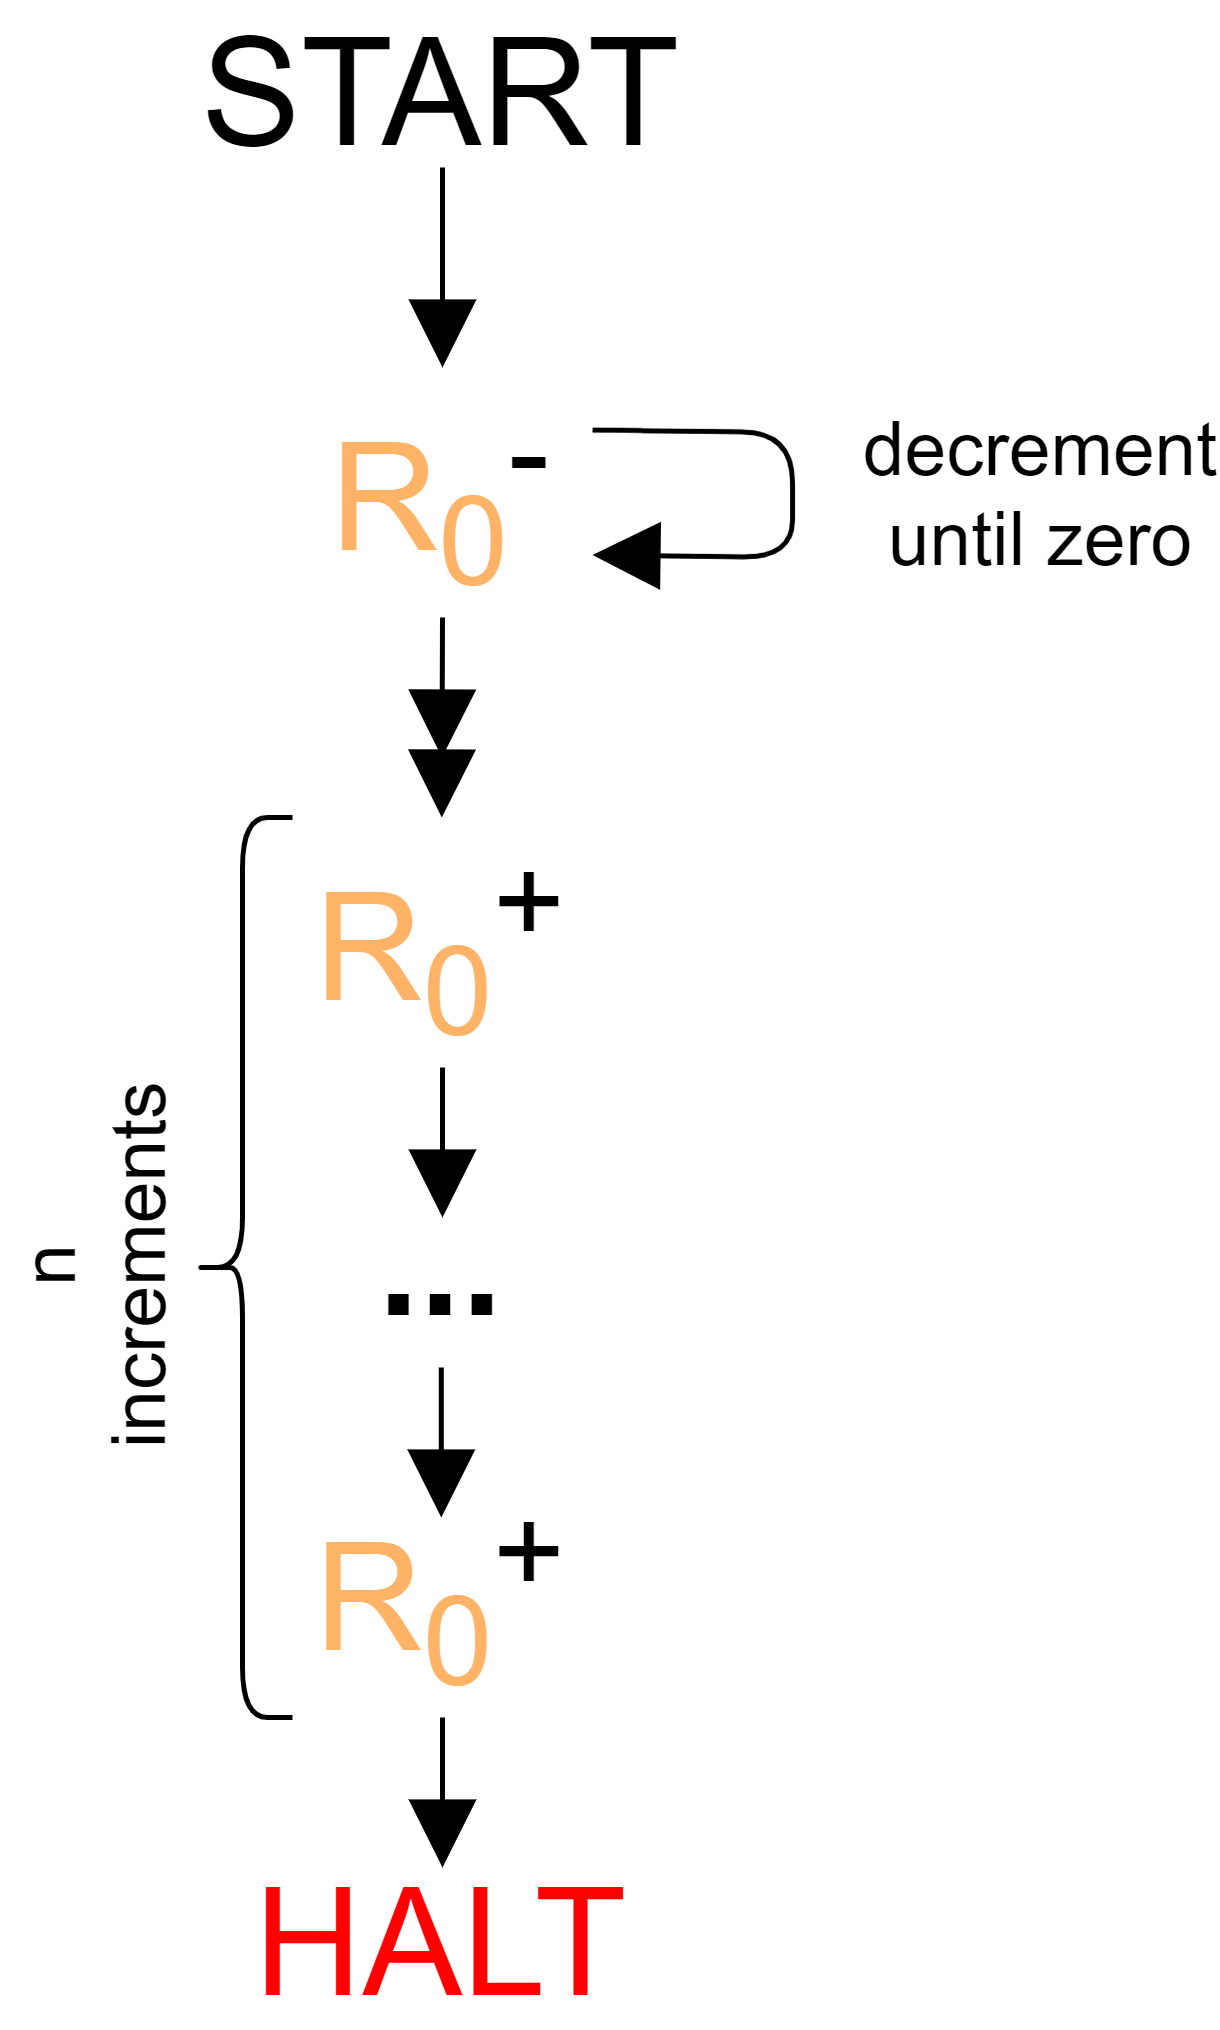
\includegraphics[scale=0.06]{register_machines/images/rm_functions/constant.drawio.png}
    \end{center}
}

\subsubsection*{Truncated Subtraction}
\trisplit{
	\[x - y \triangleq \begin{cases}
			x - y & y \leq x \\
			0     & y > x
		\end{cases}\]
	\[(r_0, r_1) \to r_0 - r_1\]
}{
	\[
		\begin{matrix*}[l]
			\instr{0}{\dec{1}{1}{2}}
			\instr{1}{\dec{0}{0}{2}}
			\instr{2}{\halt}
		\end{matrix*}
	\]
}{
    \begin{center}
        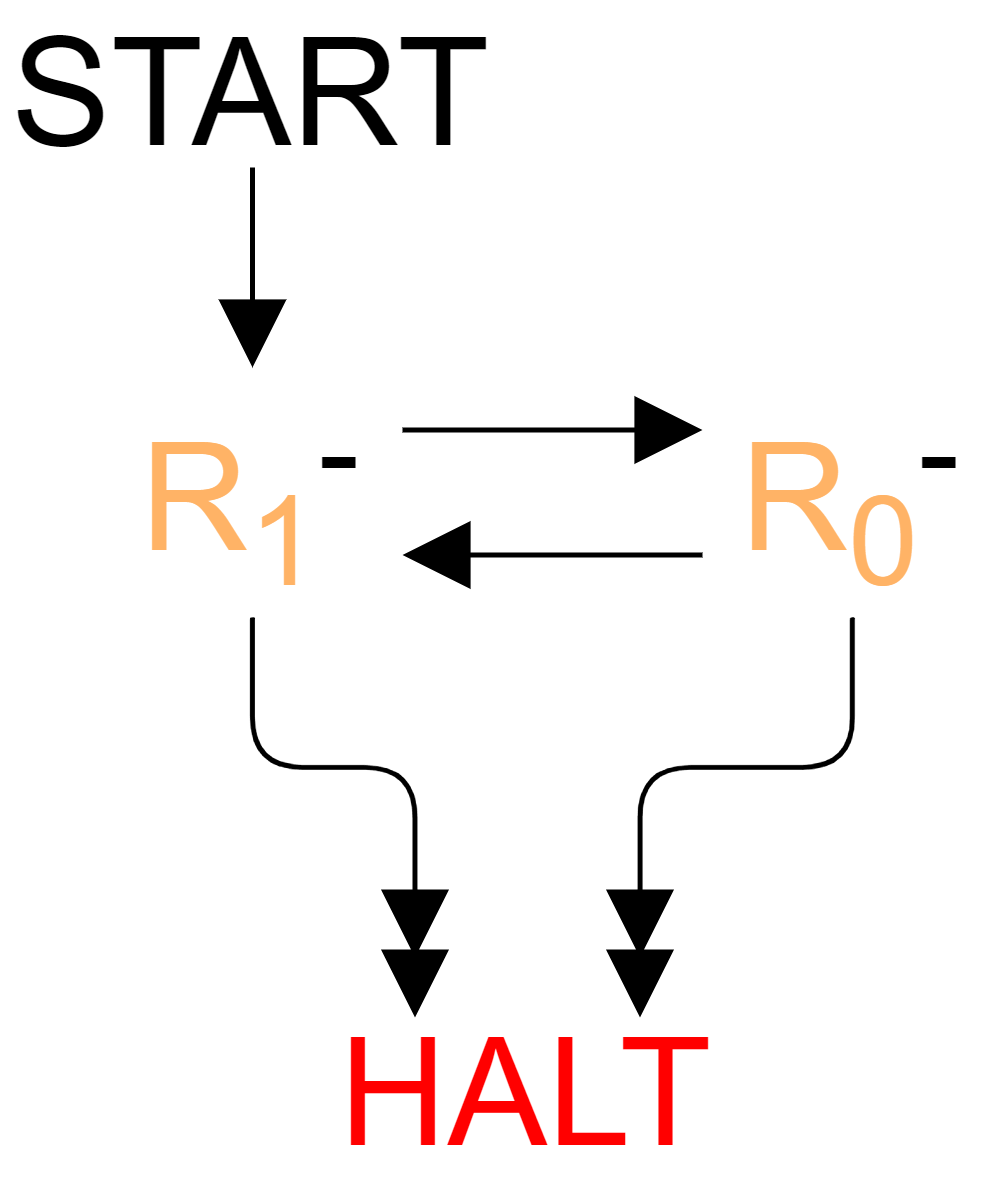
\includegraphics[scale=0.06]{register_machines/images/rm_functions/truncated_subtraction.drawio.png}
    \end{center}
}

\subsubsection*{Integer Division}
Note that this is an inefficient implementation (to make it easy to follow) we could combine the halts and shortcut the initial zero check (so we don't increment, then re-decrement).
\\ \trisplit{
	\[x \ div \ y \triangleq \begin{cases}
			\left\lfloor \cfrac{x}{y} \right\rfloor & y > 0 \\
			0                                       & y = 0 \\
		\end{cases}\]
}{
	\[
		\begin{matrix*}[l]
			\instr{0}{\dec{1}{3}{2}}
			\instr{1}{\dec{0}{1}{2}}
			\instr{2}{\halt}
			\instr{3}{\inc{1}{4}}
			\instr{4}{\dec{1}{5}{7}}
			\instr{5}{\inc{2}{6}}
			\instr{6}{\inc{3}{4}}
			\instr{7}{\dec{3}{8}{9}}
			\instr{8}{\inc{1}{9}}
			\instr{9}{\dec{2}{10}{4}}
			\instr{10}{\dec{0}{9}{11}}
			\instr{11}{\dec{4}{12}{13}}
			\instr{12}{\inc{0}{11}}
			\instr{13}{\halt}
		\end{matrix*}
	\]
}{
    \begin{center}
        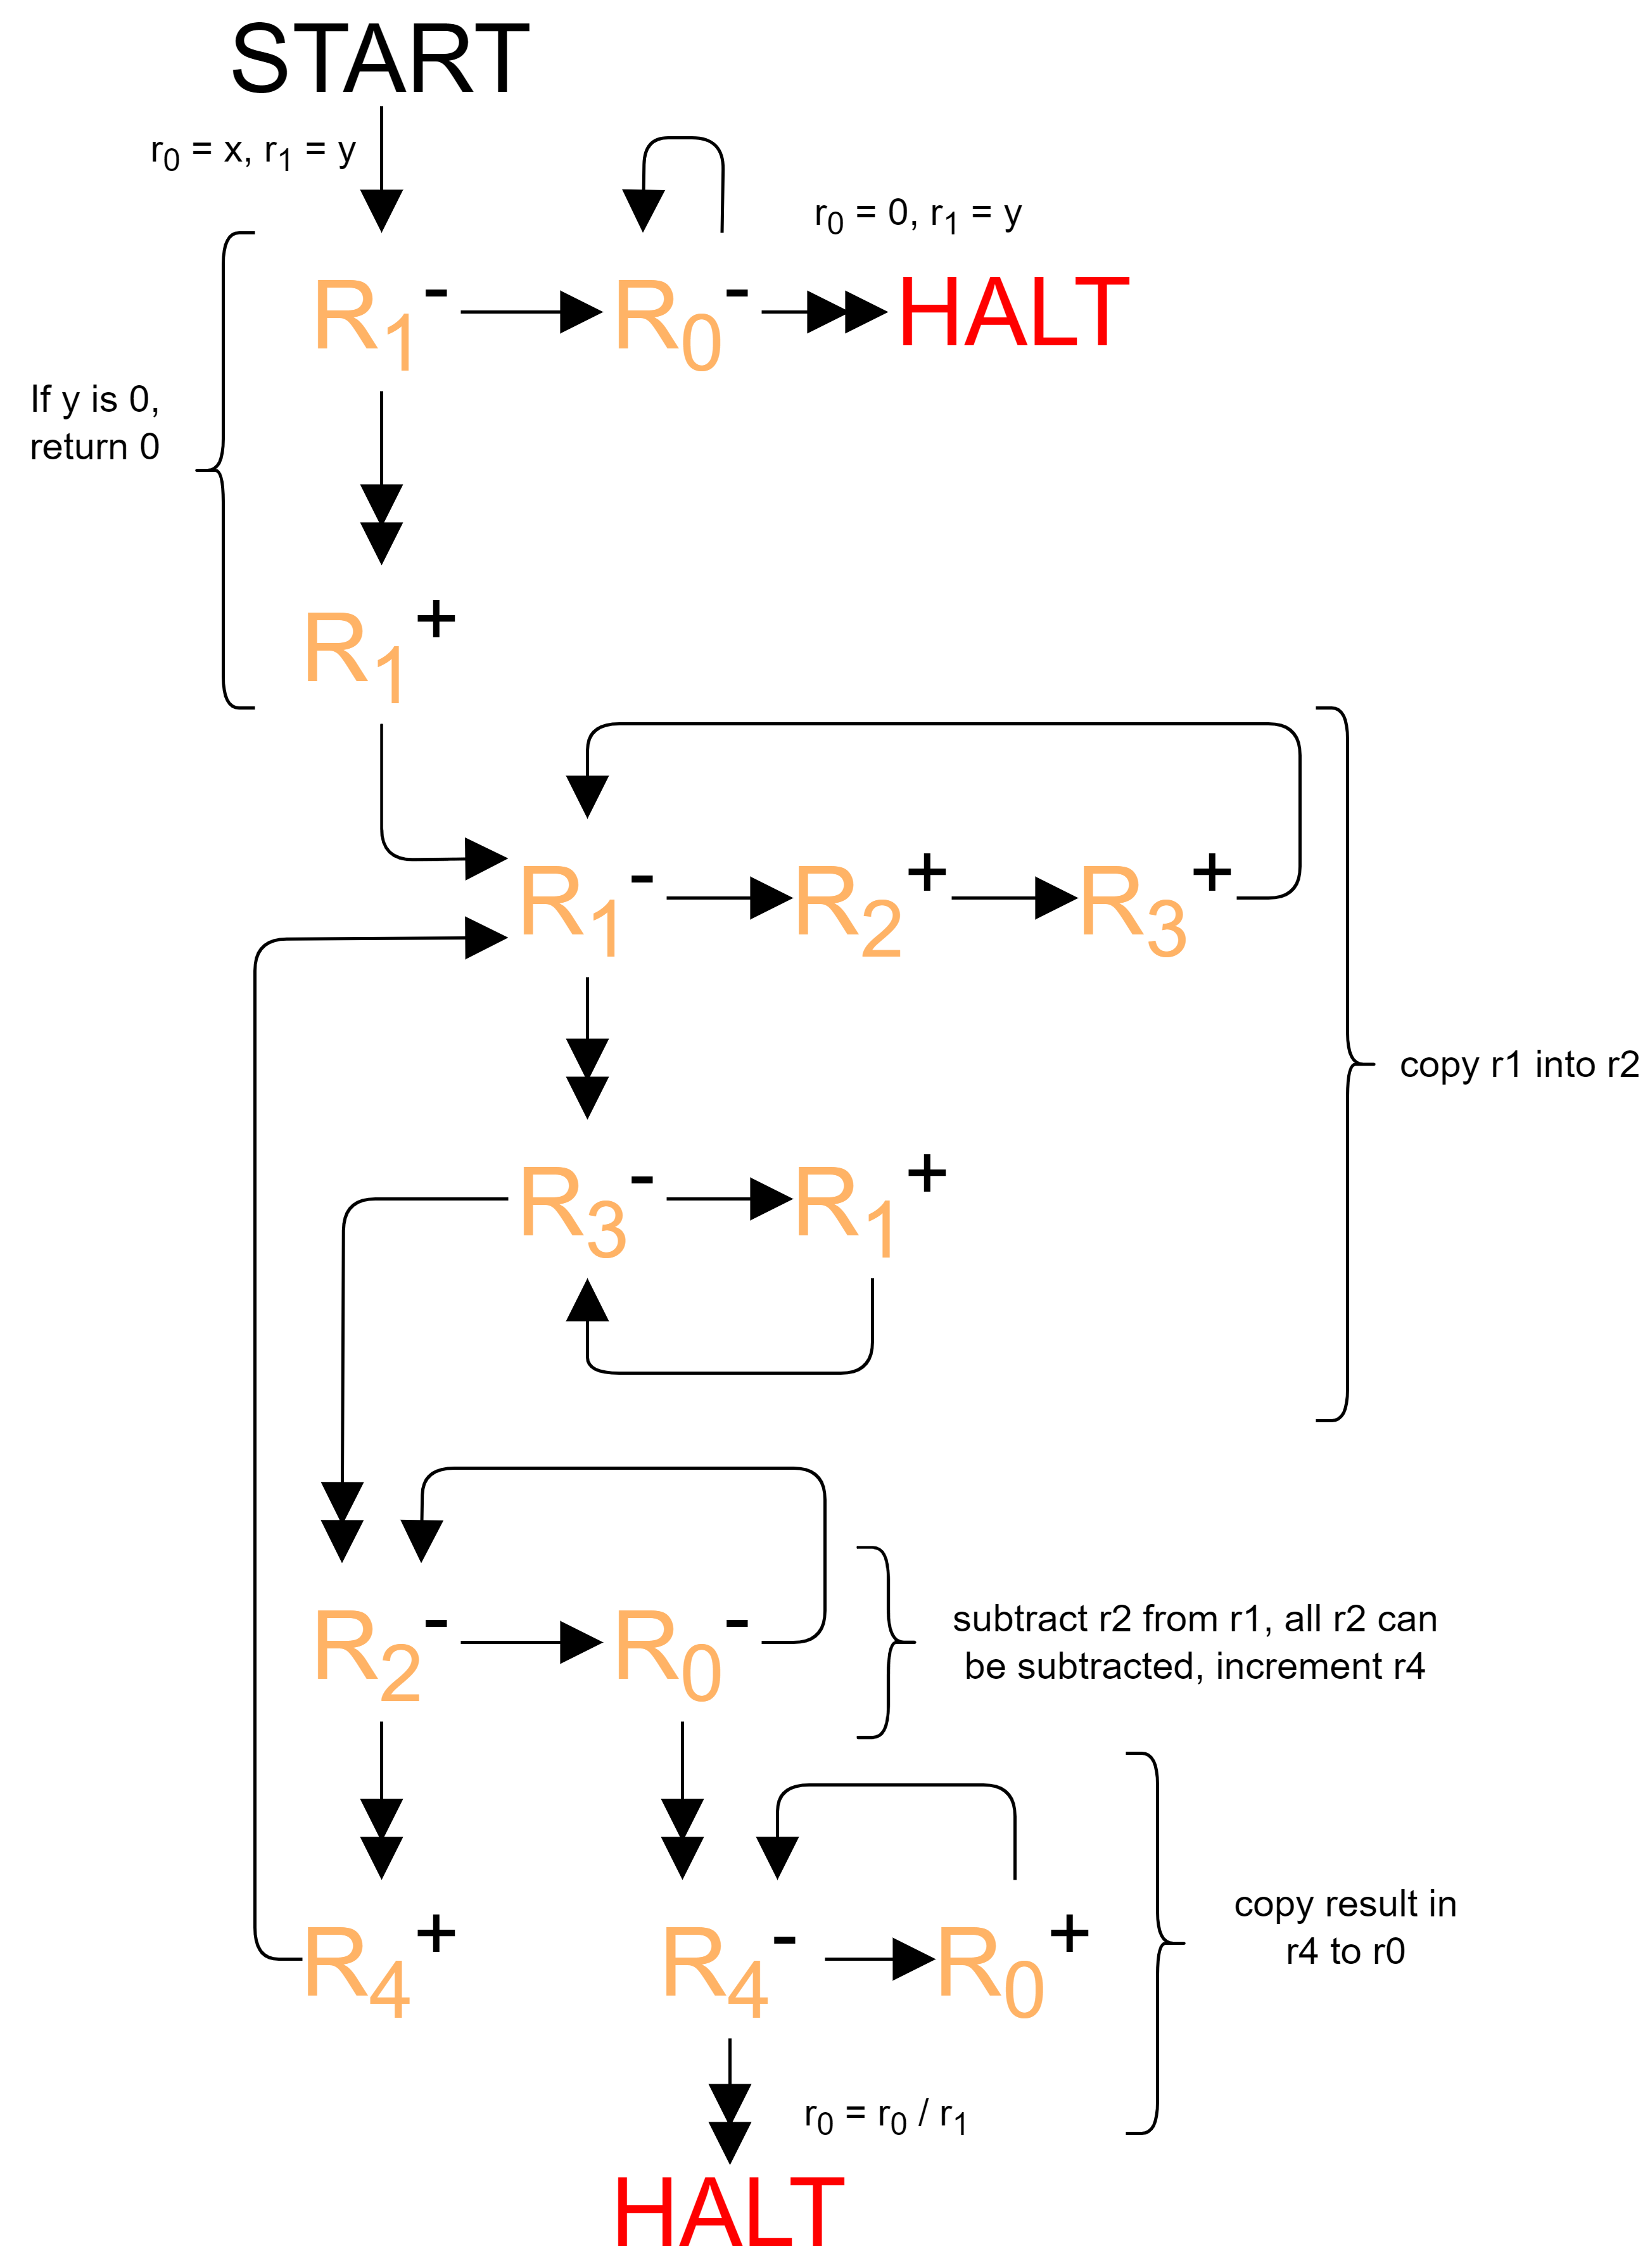
\includegraphics[scale=0.06]{register_machines/images/rm_functions/integer_division.drawio.png}
    \end{center}
}
\subsubsection*{Multiplication}
\trisplit{
	\[x \times y\]
}{
	\[
		\begin{matrix*}[l]
			\instr{0}{\dec{1}{5}{1}}
			\instr{1}{\dec{0}{1}{2}}
			\instr{2}{\dec{3}{3}{4}}
			\instr{3}{\inc{0}{2}}
			\instr{4}{\halt}
			\instr{5}{\dec{0}{6}{8}}
			\instr{6}{\inc{2}{7}}
			\instr{7}{\inc{3}{5}}
			\instr{8}{\dec{2}{9}{0}}
			\instr{9}{\inc{0}{8}}
		\end{matrix*}
	\]
}{
    \begin{center}
        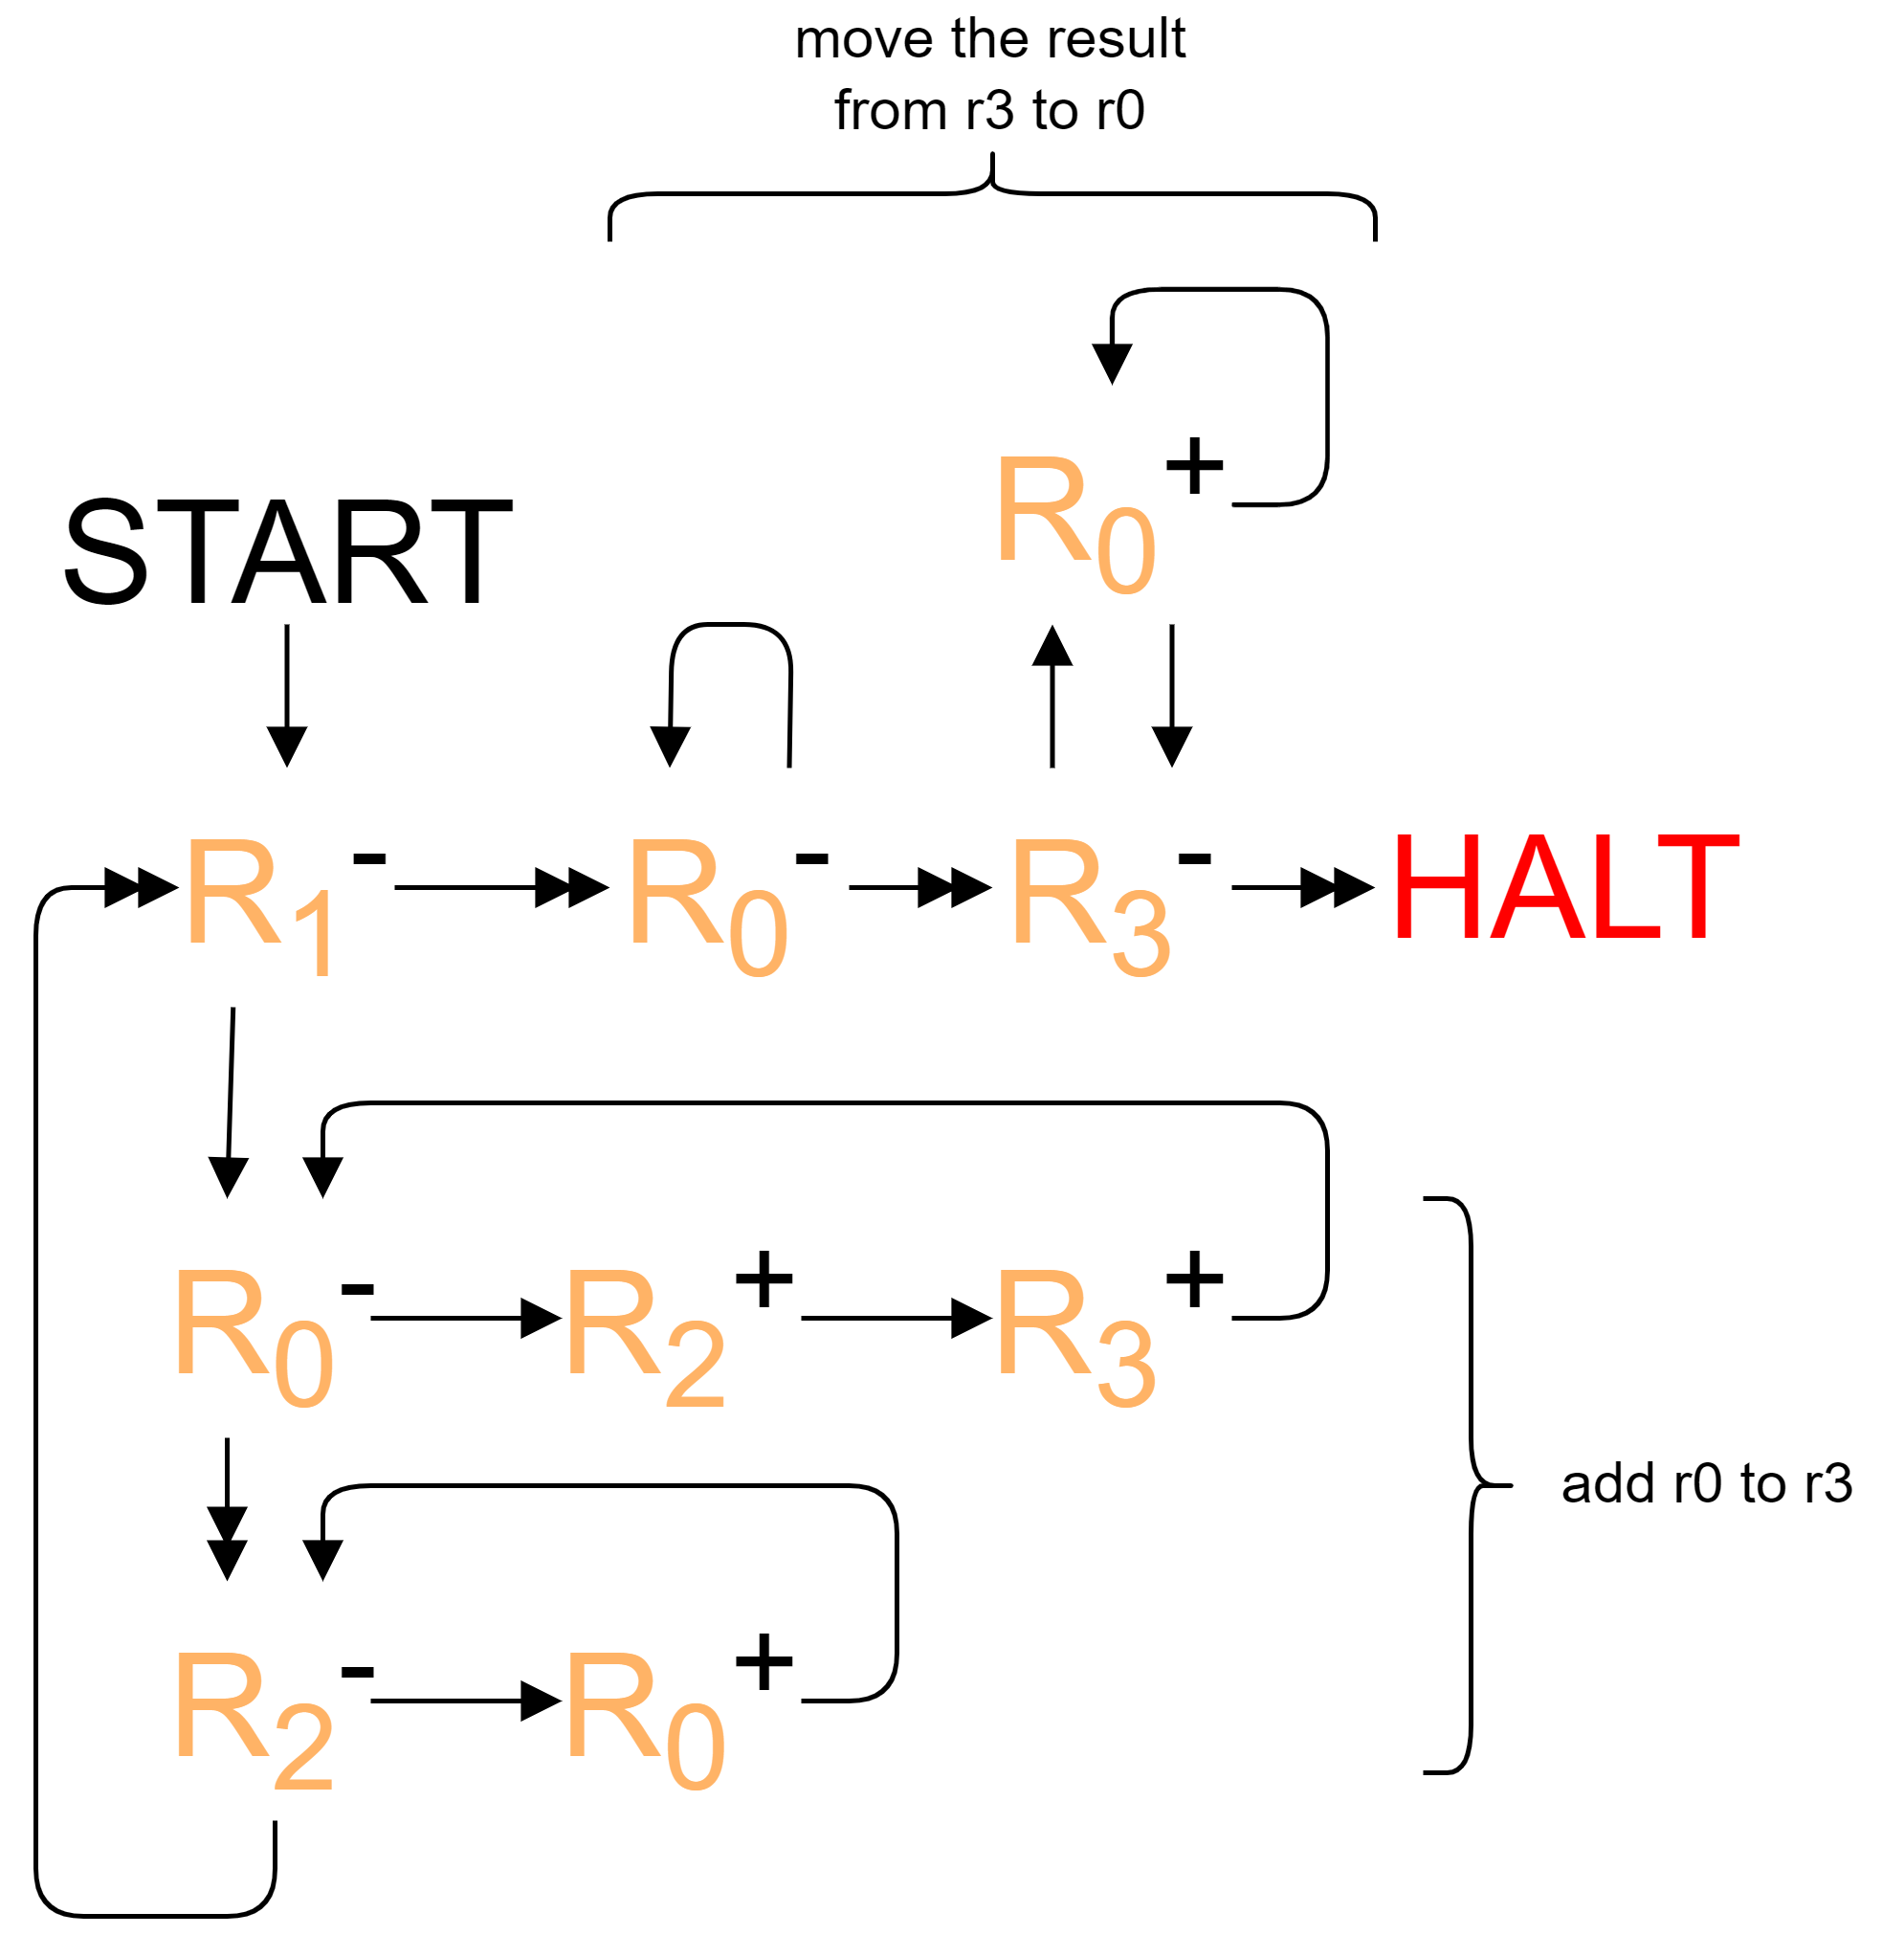
\includegraphics[scale=0.06]{register_machines/images/rm_functions/integer_multiplication.drawio.png}
    \end{center}
}
\subsubsection*{Exponent of base 2}
\trisplit{
	\[e(x) \triangleq 2^x \]
}{
	\[
		\begin{matrix*}[l]
			\instr{0}{\inc{1}{1}}
			\instr{1}{\dec{0}{5}{2}}
			\instr{2}{\dec{1}{3}{4}}
			\instr{3}{\inc{0}{2}}
			\instr{4}{\halt}
			\instr{5}{\dec{1}{6}{7}}
			\instr{6}{\inc{2}{5}}
			\instr{7}{\dec{2}{8}{1}}
			\instr{8}{\inc{1}{9}}
			\instr{9}{\inc{1}{7}}
		\end{matrix*}
	\]
}{
    \begin{center}
        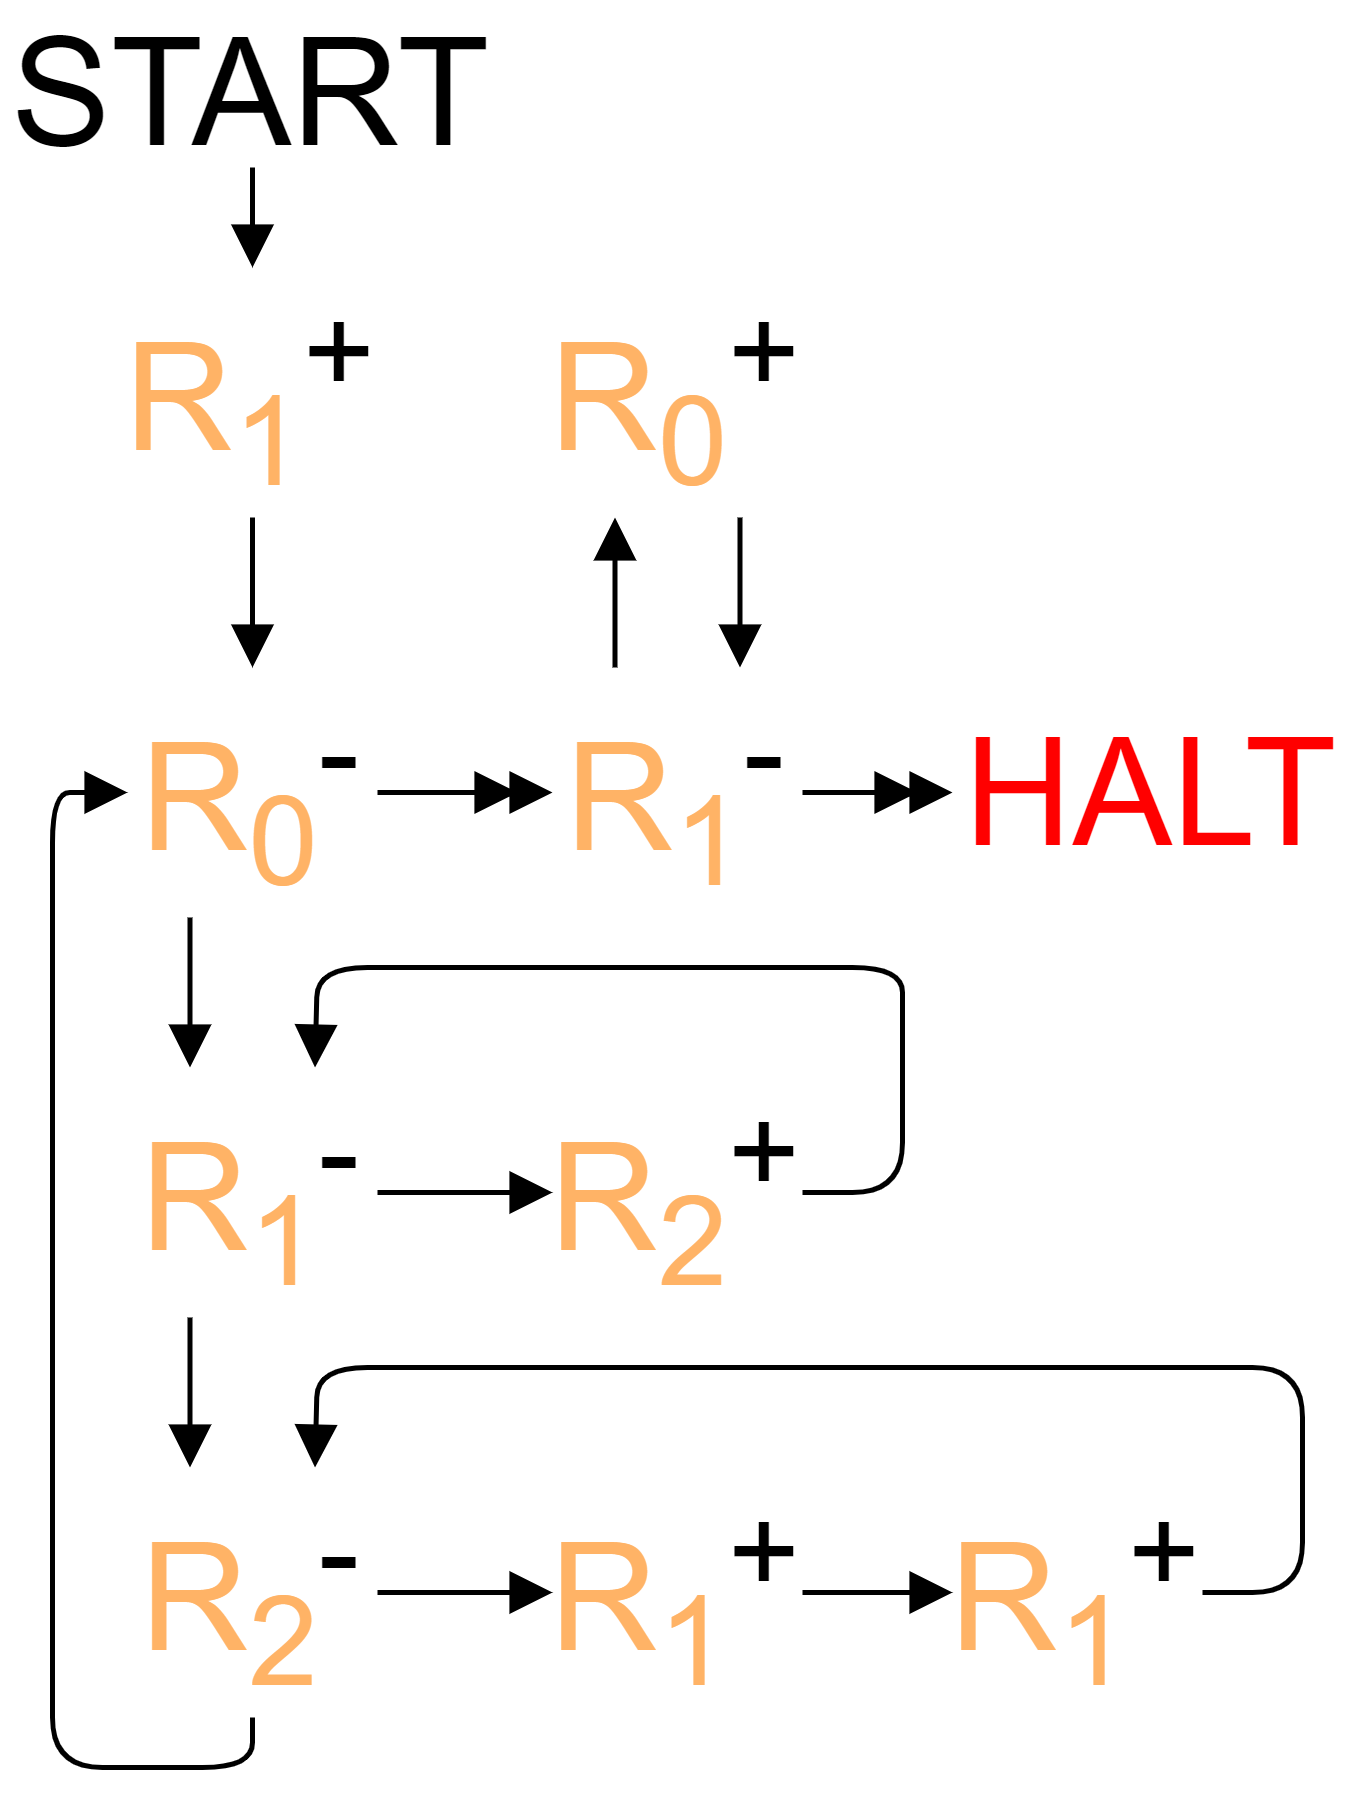
\includegraphics[scale=0.06]{register_machines/images/rm_functions/exponent_base_2.drawio.png}
    \end{center}
}

\begin{exambox}{2bi}{2021/22}
	Consider the graphical representation of a Register Machine $M$:
	\begin{center}
		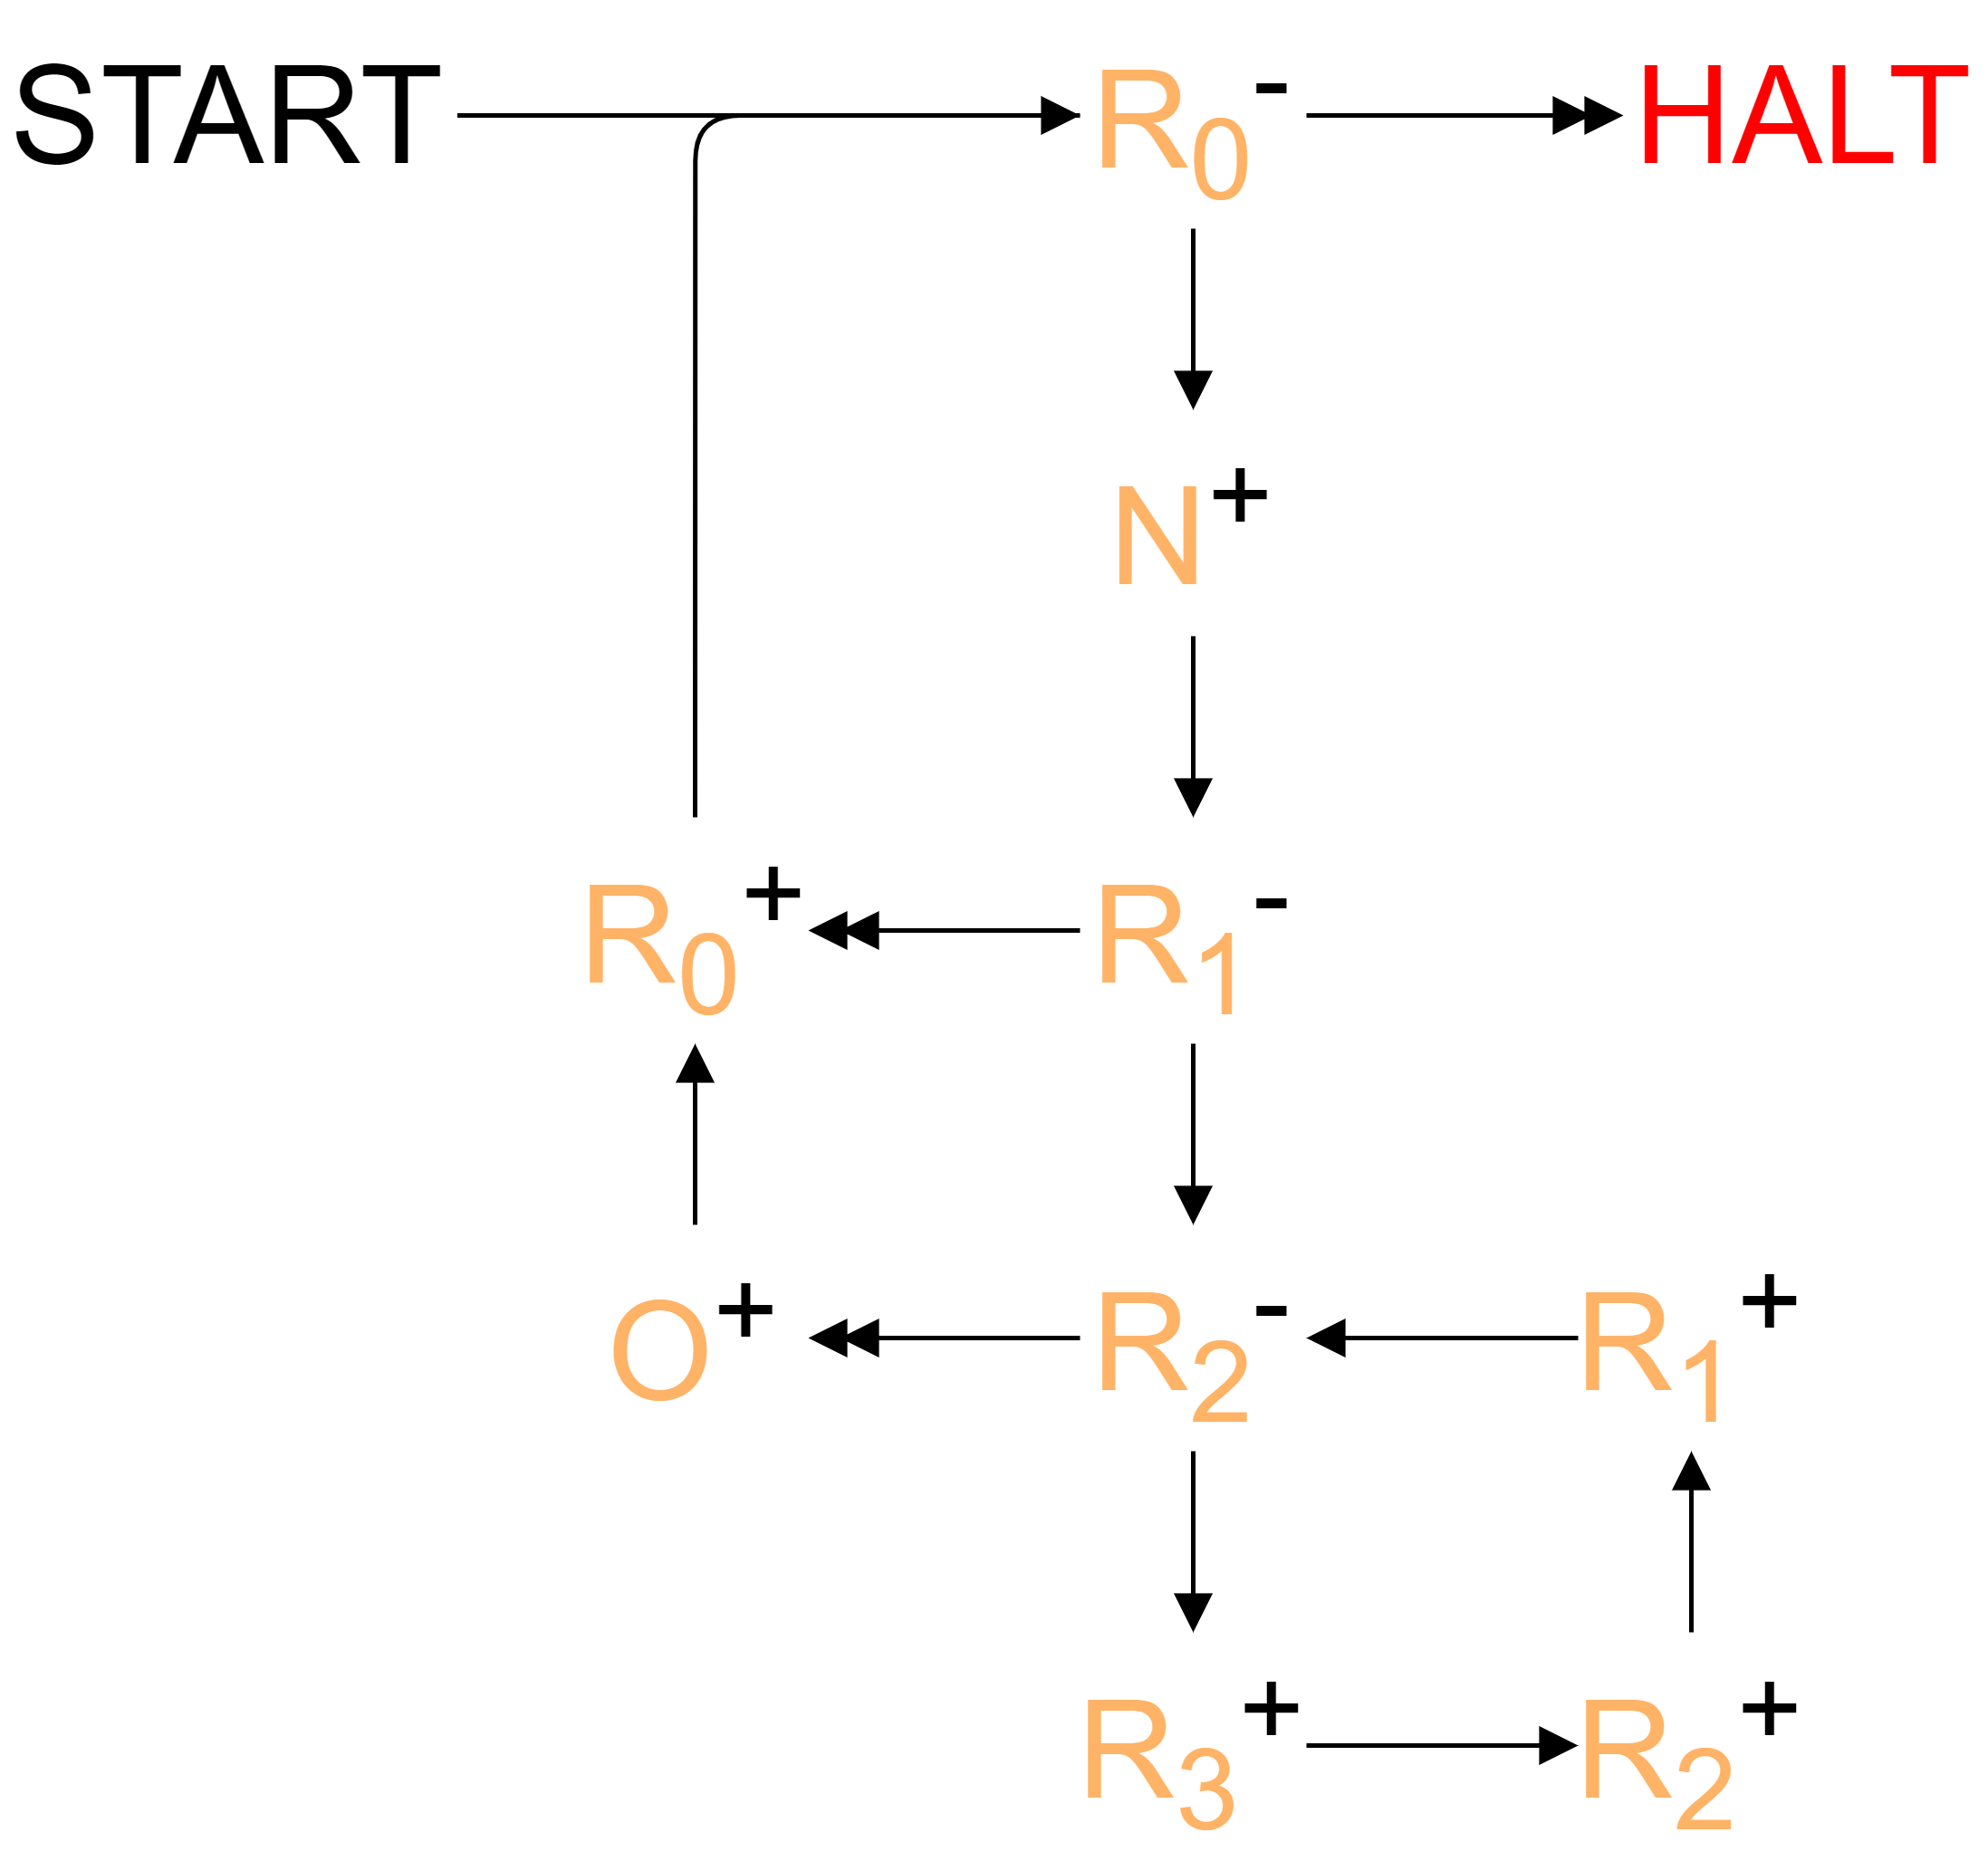
\includegraphics[width=.4\textwidth]{register_machines/images/exam_2bi_2021_2022.drawio.png}
	\end{center}
	Write down the program/code (list of instructions) for this machine using only a single $\halt$ instruction (at the end of the code).
\end{exambox}

\begin{exambox}{2bi}{2020/21}
	Describe (graphically) a Register Machine (RM) gadget which tests if $R_0$ is
	even or odd without changing the value of $R_0$ and using only RM
	instructions (no gadgets).
	\begin{center}
		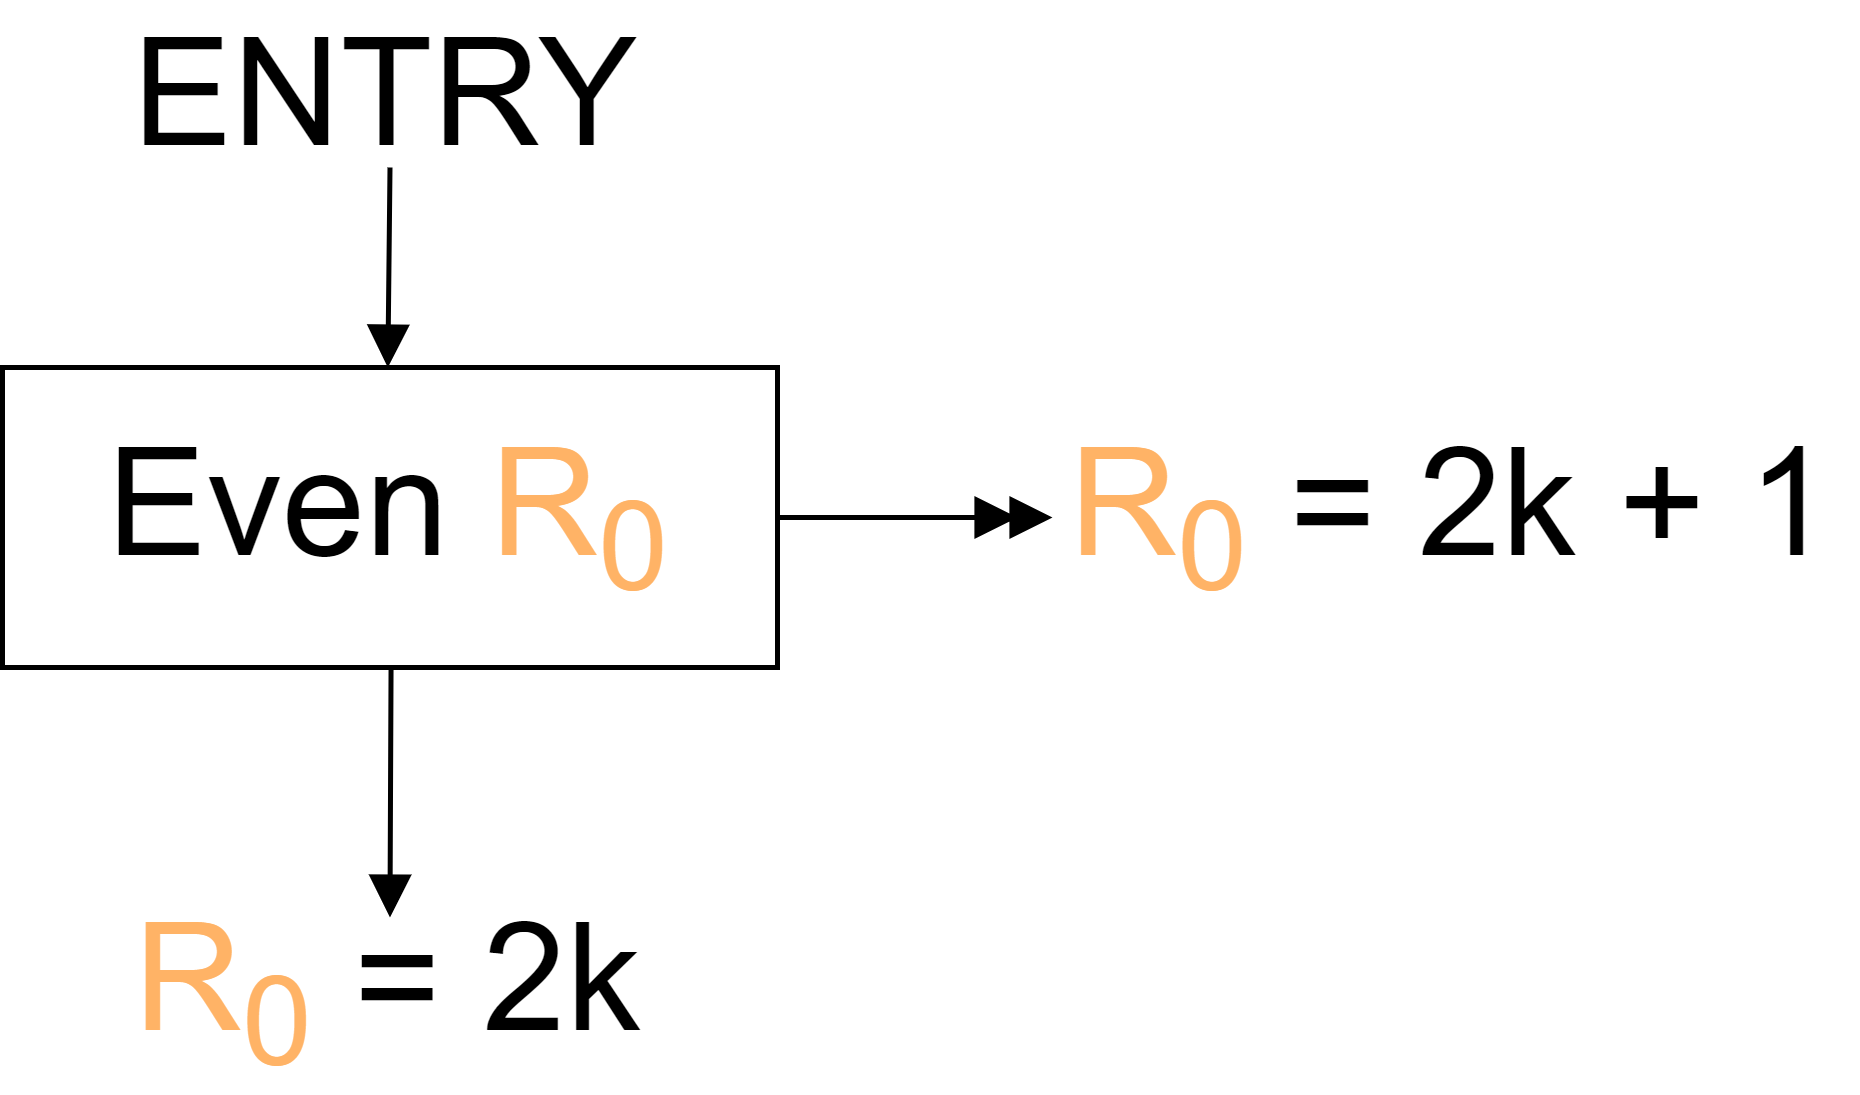
\includegraphics[width=.5\textwidth]{register_machines/images/exam_2bi_2020_2021.drawio.png}
	\end{center}
\end{exambox}

\begin{exambox}{2bii}{2020/21}
	\textit{Note: This question contains corrections from the original paper}
	\\
	\\ Consider the graphical representation of register machine $M$:
	\begin{center}
		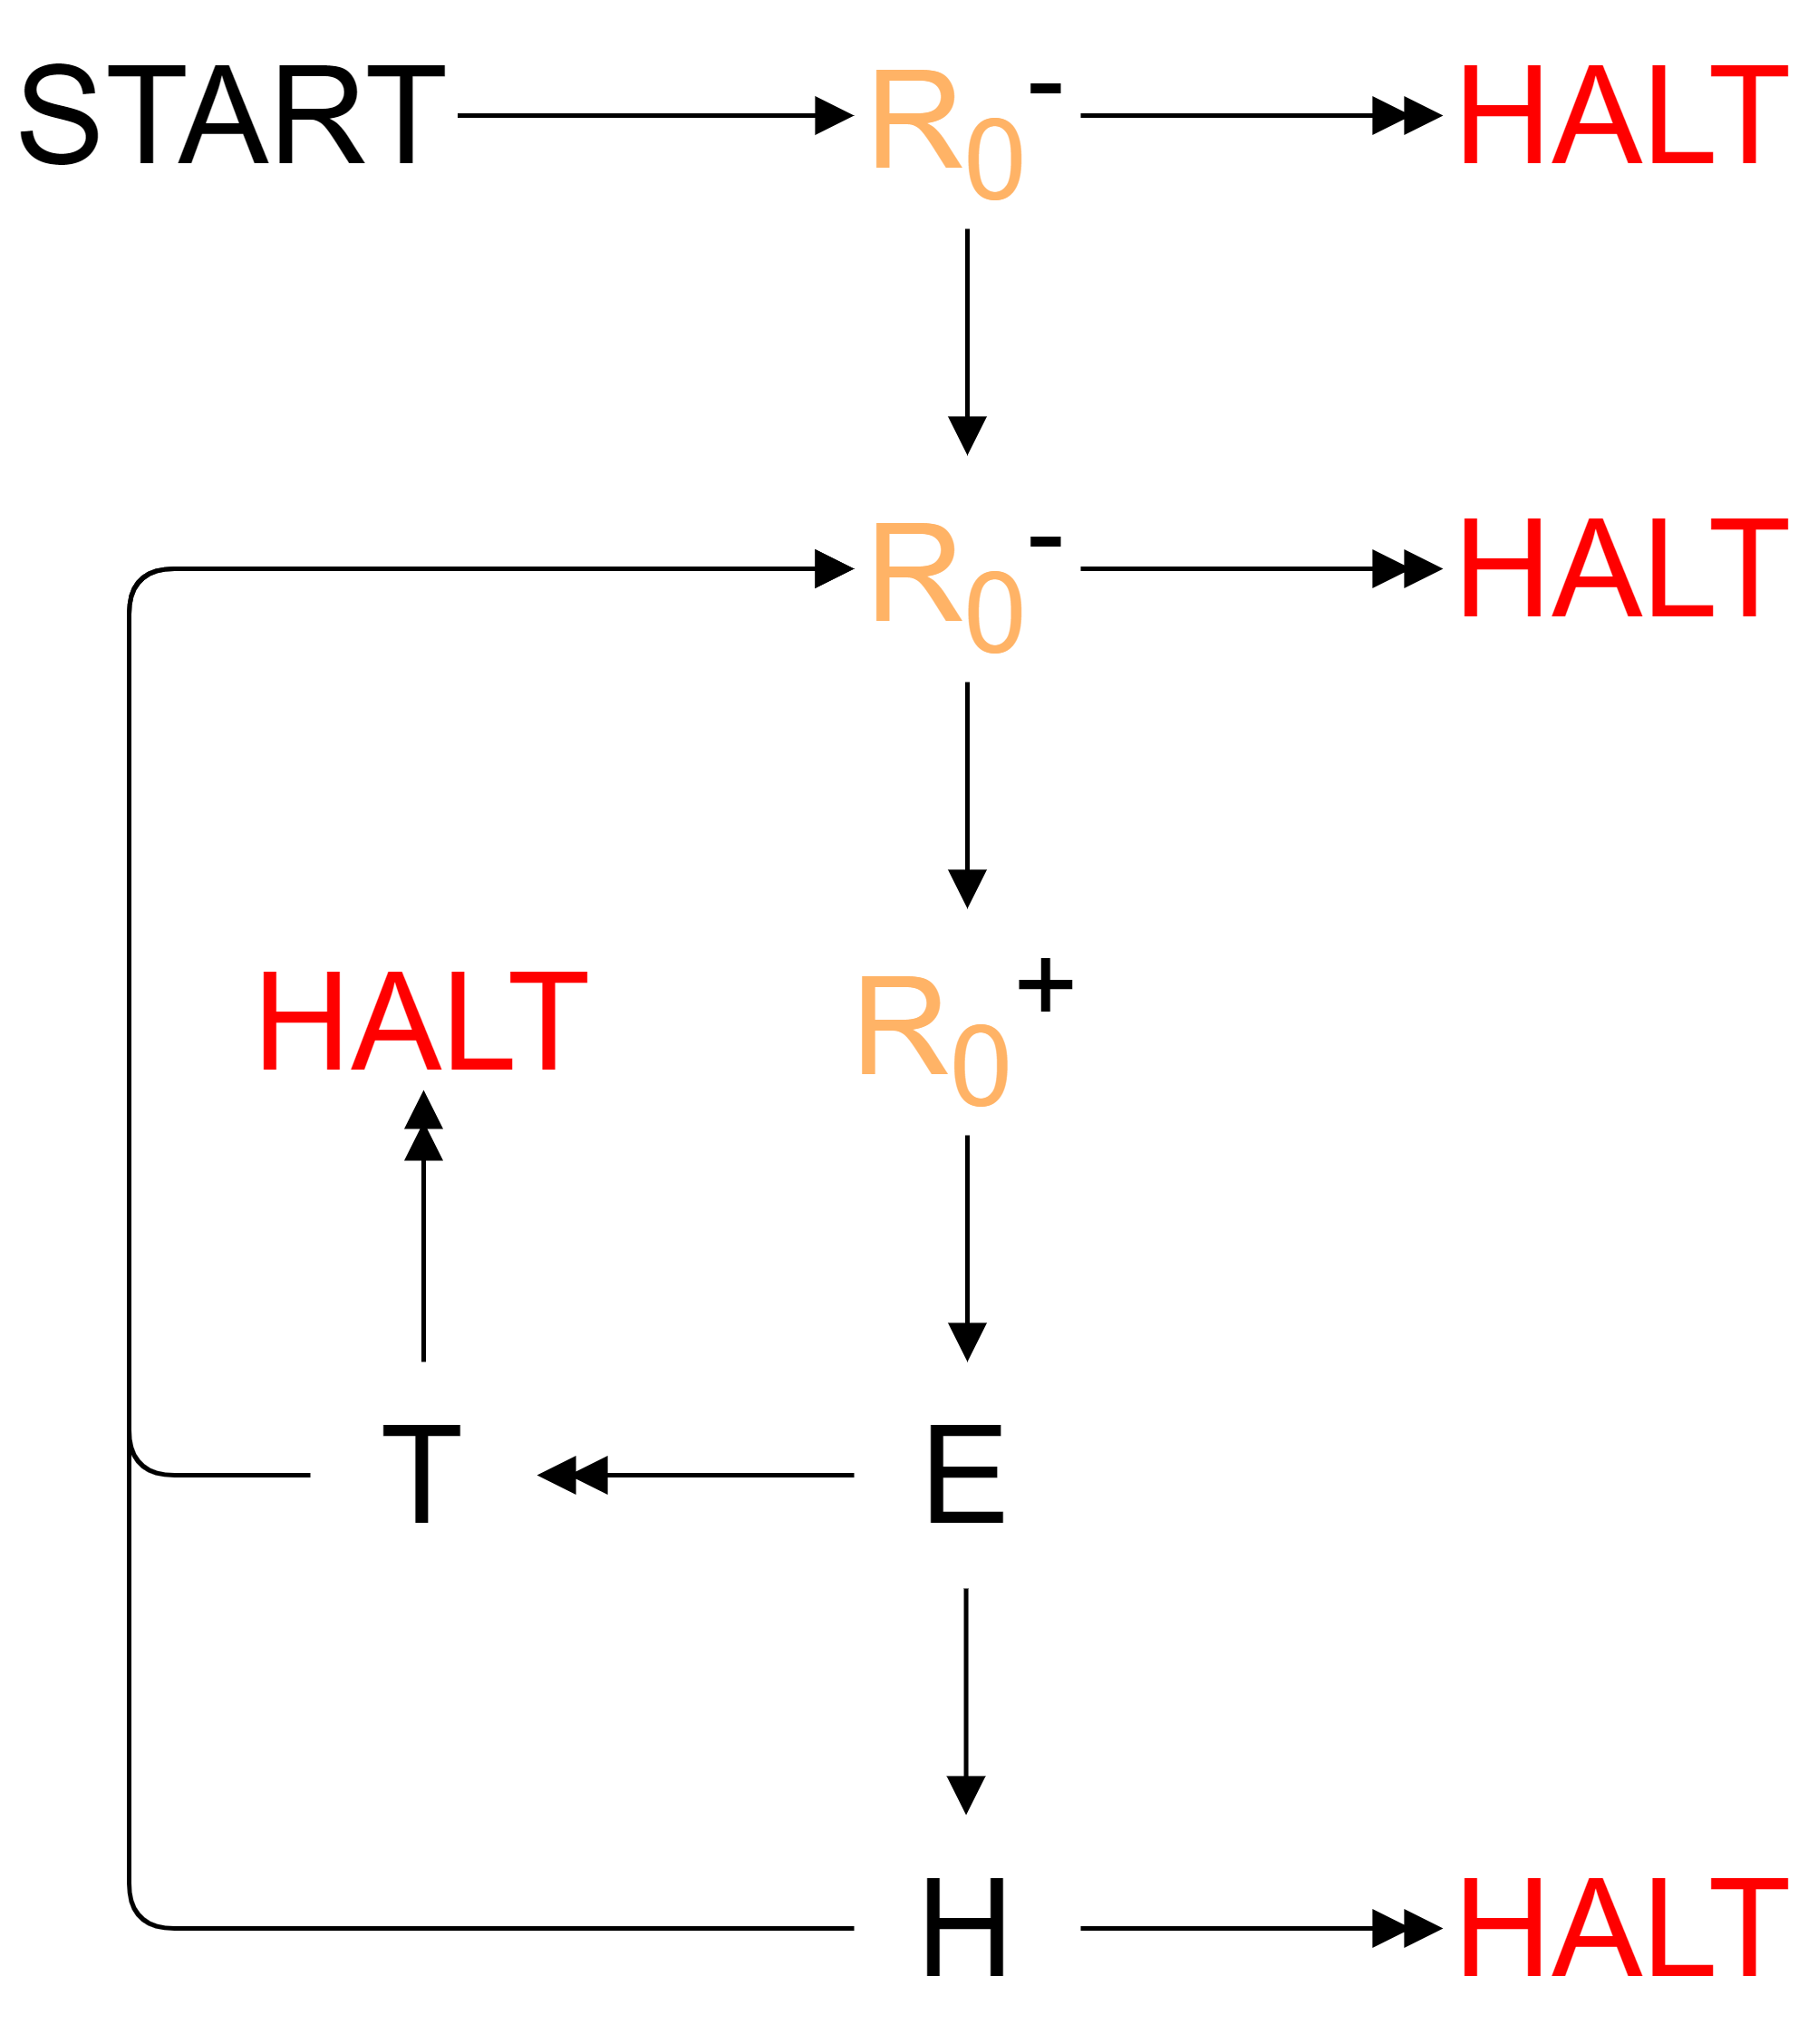
\includegraphics[width=.4\textwidth]{register_machines/images/exam_2bii_2020_2021.drawio.png}
	\end{center}
	Take for $E \equiv R_1^-$, $H \equiv R_2^-$ and $T \equiv R_0^-$.
	\\
	\\ Write down the program, code or list of instructions for this machine using only a single $\halt$ instruction (at end of the code).
\end{exambox}

\section{Encoding Programs as Numbers}

\begin{definitionbox}{Halting Problem}
	Given a set $S$ of pairs $(A,D)$ where $A$ is an algorithm and $D$ is some input data $A$ operates on ($A(D)$).
	\\
	\\ We want to create some algorithm $H$ such that:
	\[H(A,D) \triangleq \begin{cases}
			1 & A(D)\downarrow \\
			0 & otherwise
		\end{cases}\]
	Hence if $A(D)\downarrow$ then $A(D)$ eventually halts with some result.
	\\
	\\ We can use proof by contradiction to show no such algorithm $H$ can exist.
	\\
	\\ Assume an algorithm $H$ exists:
	\[B(p) \triangleq \begin{cases}
			halts   & H(p(p)) = 0 \ \text{  ($p(p)$ does not halt)} \\
			forever & H(p(p)) = 1 \ \text{  ($p(p)$ halts)}         \\
		\end{cases}\]
	Hence using $H$ on any $B(p)$ we can determine if $p(p)$ halts ($H(B(p)) \Rightarrow \neg H(p(p))$).
	\\
	\\ Now we consider the case when $p = B$.
    \begin{center}
        \begin{tabular}{l p{.8\textwidth}}
            \textbf{$B(B)$ halts} & Hence $B(B)$ does not halt. Contradiction! \\
            \textbf{$B(B)$ does not halt} & Hence $B(B)$ halts. Contradiction! \\
        \end{tabular}
    \end{center}
	Hence by contradiction there is not such algorithm $H$.
\end{definitionbox}
In order to reason about programs consuming/running programs (as in the halting problem), we need a way to encode programs as data. Register machines use natural numbers as values for input, and hence we need a way to encode any register machine as a natural number.
\subsection{Pairs}
\begin{center}
	\begin{tabular}{r l c l}
		$\langle\langle x, y \rangle\rangle $ & $= 2^x(2y + 1)$     & $y \ 1 \ 0_1 \dots 0_x$ & Bijection between $\mathbb{N} \times \mathbb{N}$ and $\mathbb{N}^+ = \{n \in \mathbb{N} | n \neq 0\}$ \\
		$\langle x, y \rangle $               & $= 2^x(2y + 1) - 1$ & $y \ 0 \ 1_1 \dots 1_x$ & Bijection between $\mathbb{N} \times \mathbb{N}$ and $\mathbb{N}$                                     \\
	\end{tabular}
\end{center}

\begin{exambox}{2a}{2021/22}
	Either state your birthday or take today's date as $B = YYMMDD$ (i.e. last two
	digits of the year, two digits representing month and day each) and determine the
	pair, the list, and the Register Machine (RM) instruction it represents, i.e. for
	which pair $x, y$ do we have $\langle \langle x, y \rangle \rangle = B$, for which list $\ell$ of numbers do we get
	$\ulcorner \ell \urcorner = B$, and for which Register Machine instruction $I$ do we have that
	$\ulcorner I \urcorner = B$?  
	\\
	\\ Show your work, e.g. binary representation of your $B$, etc.
\end{exambox}
\begin{exambox}{2a}{2020/21}
	State your $CID$ and determine the pair, the list, and the Register Machine (RM)
	instruction it represents, i.e. for which pair $x, y$ do we have $\langle \langle x, y \rangle \rangle = $ CID, for
	which list $\ell$ of numbers do we get $\ulcorner ell \urcorner = CID$, and for which register-machine
	instructions $I$ do we have that $\ulcorner I \urcorner = CID$? 
	\\
	\\ Show your work, e.g. binary representation of your $CID$, etc.
	\\
	\\ Add eight to your $CID$, i.e. consider $CID+8$, and repeat these three decodings.
	\\
	\\ Can one be sure that very student in class can (in principle) decode their $CID$s as requested?
\end{exambox}

\subsection{Lists}
We can express lists and right-nested pairs.
\[[x_1, x_2, \dots, x_n] = x_1:x_2:\dots:x_n = (x_1, (x_2, (\dots, x_n) \dots ))\]
We use zero to define the empty list, so must use a bijection that does not map to zero, hence we use the pair mapping $\langle\langle x,y \rangle\rangle$.
\[l : \begin{cases}
		\ulcorner [] \urcorner \triangleq 0                                                                            \\
		\ulcorner x_1 :: l_{inner} \urcorner \triangleq \langle\langle x, \ulcorner l_{inner} \urcorner \rangle\rangle \\
	\end{cases}\]
Hence:
\[\ulcorner x_1, \dots, x_n \urcorner = \langle\langle x_1 , \langle\langle \dots, x_n\rangle\rangle \dots \rangle\rangle\]
\subsection{Instructions}
\[\begin{split}
		\ulcorner \inc{i}{n} \urcorner &= \langle\langle 2i, n \rangle\rangle \\
		\ulcorner \dec{i}{n}{m} \urcorner &= \langle\langle 2i + 1, \langle n,m \rangle \  \rangle\rangle \\
		\ulcorner \halt \urcorner &= 0 \\
	\end{split}\]
\subsection{Programs}
Given some program:
\[\ulcorner \left( \begin{matrix*}[l]
			\instr{0}{instruction_0}
			\vdots & \vdots \\
			\instr{n}{instruction_n}
		\end{matrix*} \right) \urcorner = \ulcorner [\ulcorner instruction_0 \urcorner, \dots, \ulcorner instruction_n \urcorner] \urcorner\]

\begin{sidenotebox}{Tools}
	In order to simplify checking workings, a basic python script for running, encoding and decoding register machines is provided (also available in the notes repository).
	\begin{itemize}
		\item It is designed to be used in the python shell, to allow for easy manipulation, storing, etc of register machines, encoding/decoding results.
		\item It also produces latex to show step-by-step workings for calculations.
	\end{itemize}
	Have a go at making your own register machine encode/decode and simulation in your language of choice!
\end{sidenotebox}
\section{Gadgets}
\begin{definitionbox}{Register Machine Gadget}
	A gadget is a partial register machine graph, used as components in more complex programs, that can be composed into larger register machines or gadgets.
	\begin{itemize}
		\item Has a single $ENTRY$ (much like $START$).
		\item Can have many $EXIT$ (much like $\halt$).
		\item Operates on registers specified in the name of the gadget (e.g \textit{"Add $\reglabel{1}$ to $\reglabel{2}$"}).
		\item Can use scratch registers (assumed to be zero prior to gadget and set to zero by the gadget before it exits - allows usage in loops)
		\item We can rename the registers used in gadgets (simply change the registers used in the name (\textit{push $\reglabel{0}$ to $\reglabel{1}$ $\to$ push $\regtemp{X}$ to $\regtemp{Y}$}), and have all scratch registers renamed to registers unused by other parts of the program)
    \end{itemize}
	For example we can create several gadgets in terms of registers that we can rename.
    \begin{center}
        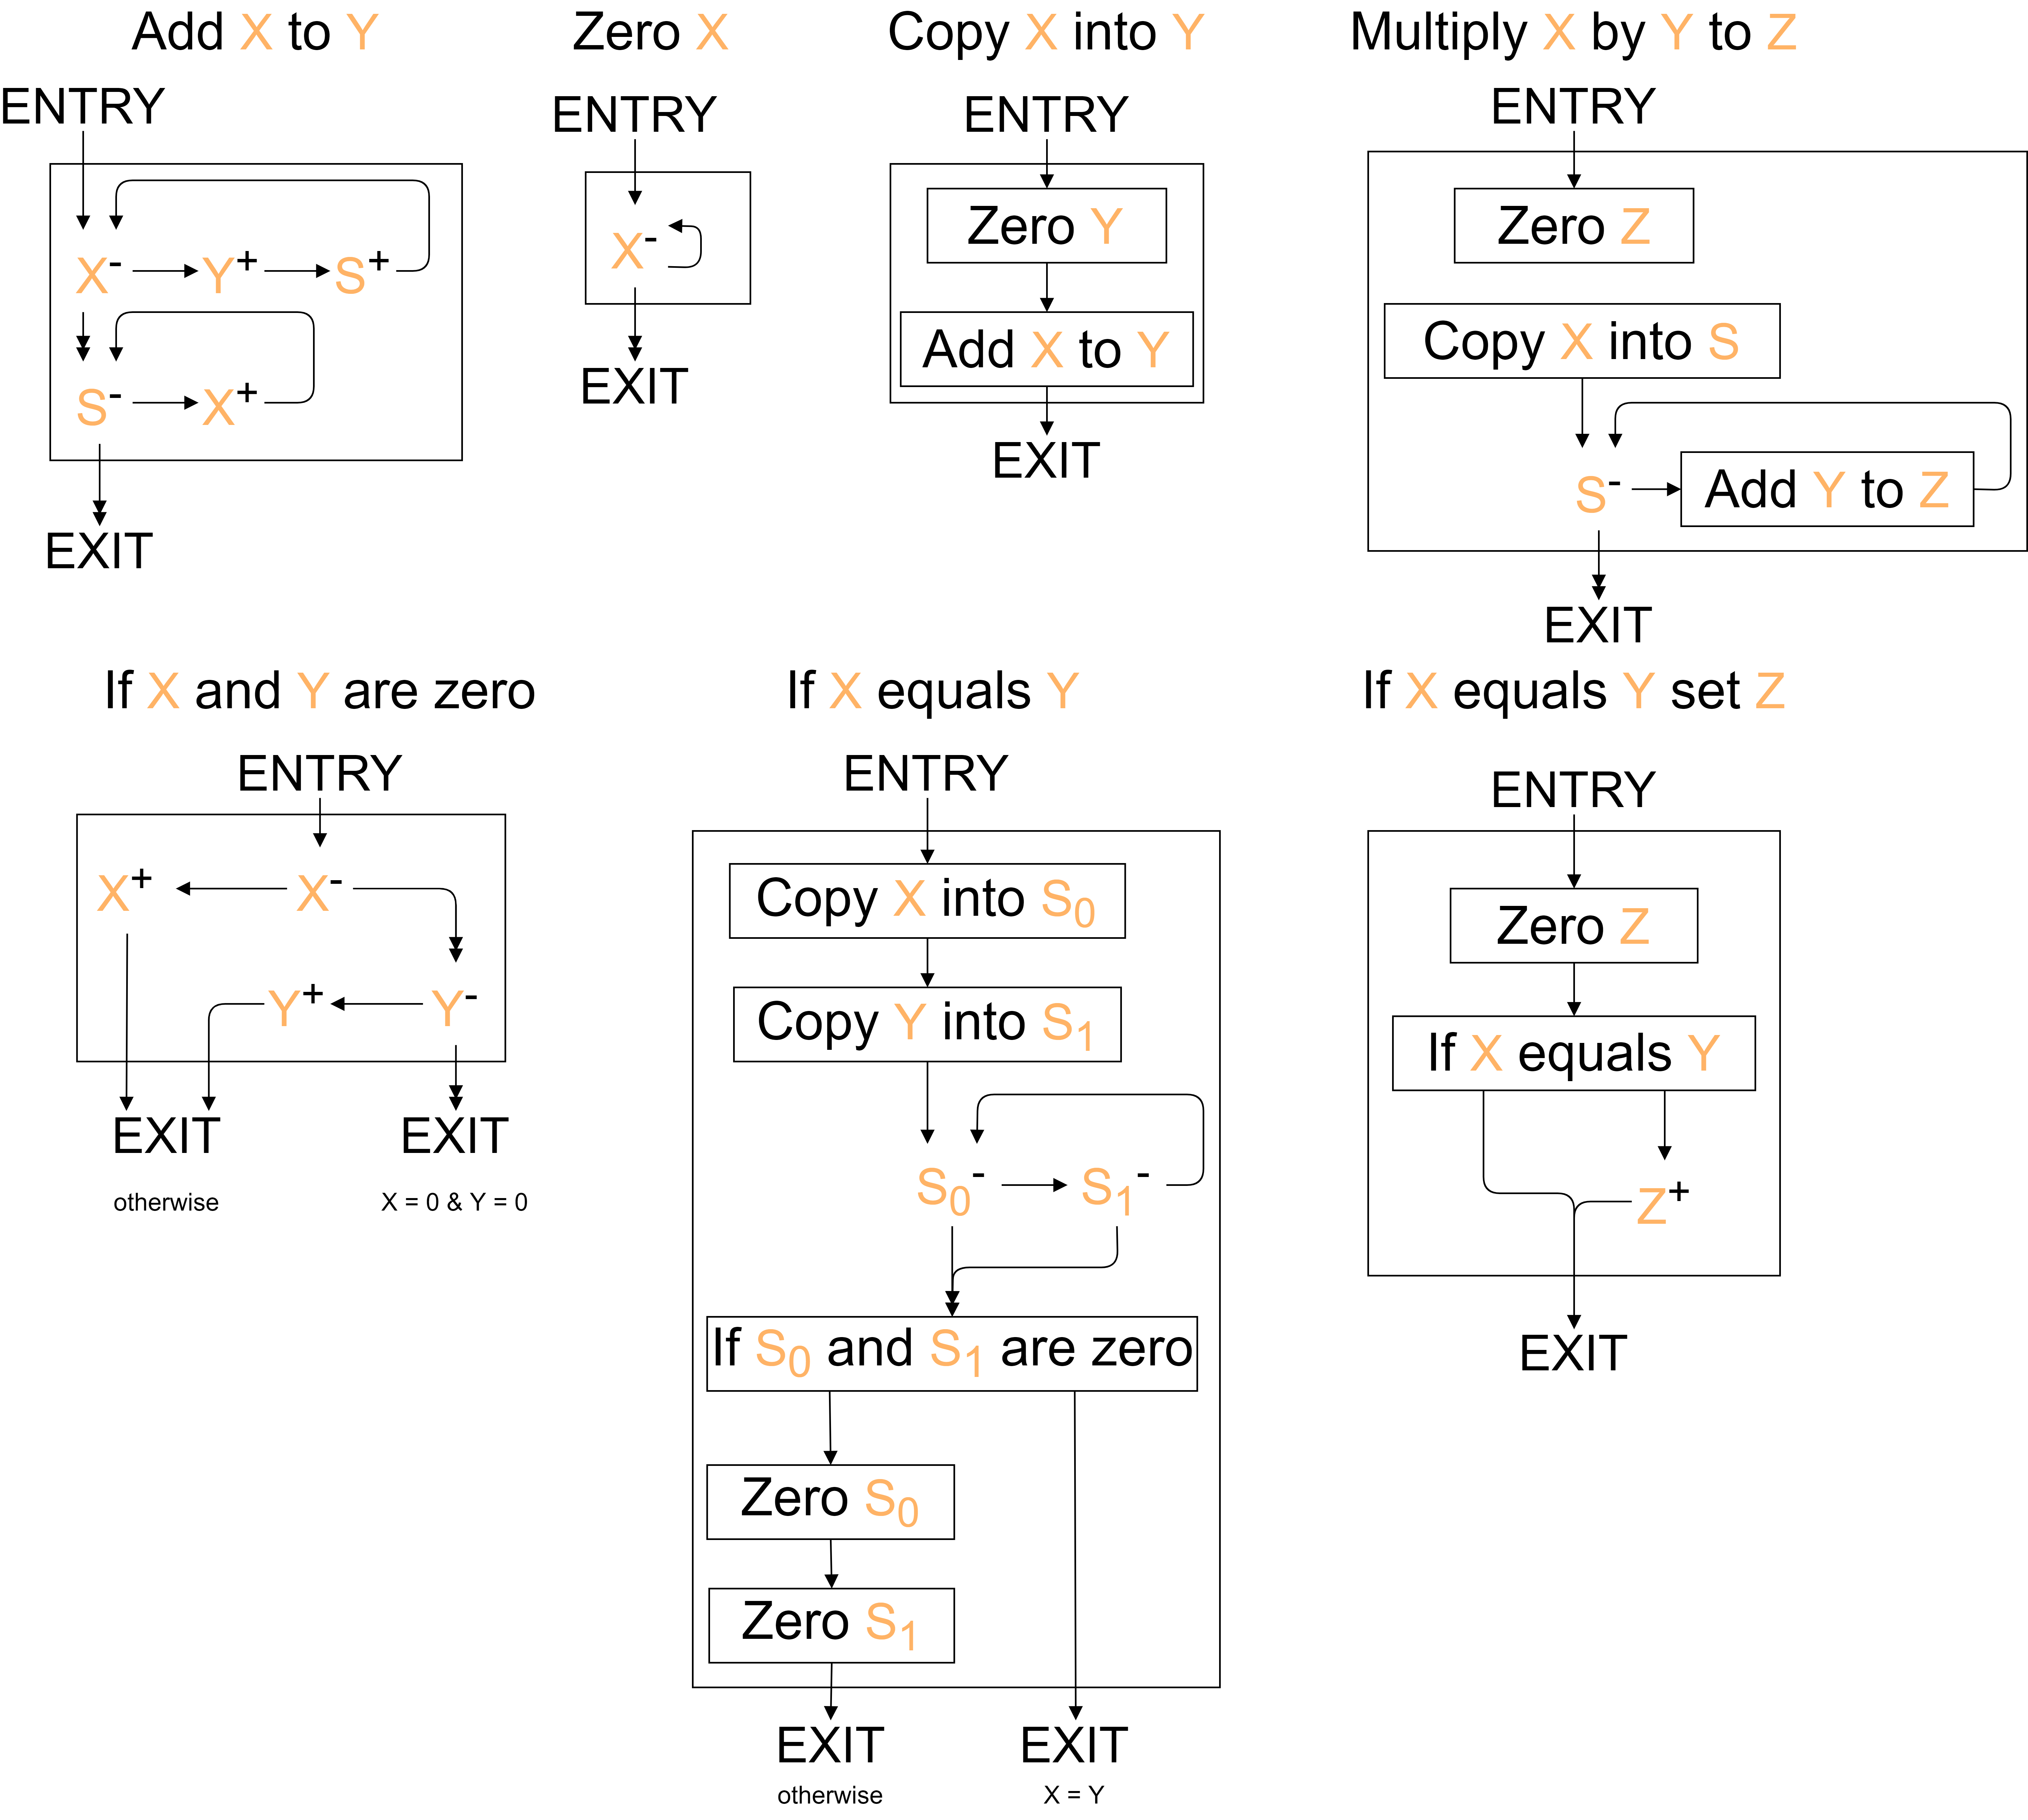
\includegraphics[width=0.9\textwidth]{register_machines/images/gadget.drawio.png}
    \end{center}
	And then can use these to create larger programs.
\end{definitionbox}

\begin{exambox}{2bii}{2021/22}
	\textit{\dots continued from question Q2bi - 2021/22}
	\\
	\\ Replace some instructions by gadgets as follows:
	\[\begin{split}
		R_0^+ & \text{ by copy } N \text{ to } O \\
		N^+   & \text{ by copy } Y \text{ to } N \\
		O^+   & \text{ by push } X \text{ to } O \\
	\end{split} \qquad \begin{split}
		R_1^- & \text{ by pop }  O \text{ to } R_1 \\
		R_2^- & \text{ by pop }  O \text{ to } R_2 \\
		R_3^+ & \text{ by add }R_2 \text{ to } R_1 \\
	\end{split} \qquad \begin{split}
		R_2^+ & \text{ by push }R_1 \text{ to } N \\
		R_1^+ & \text{ by copy } R_2 \text{ to } R_1 \\
		\\
	\end{split}\]
	where for pop gadgets the \textit{empty} exit is identified with $\twoheadrightarrow$  and \textit{done}
	with $\to$ and where we have additional registers: $X$ with (constant) value $1$
	and $Y$ with (constant) value $2$.
	\\
	\\ Draw the graphical representation of the resulting RM and describe its
	execution with initially: $R_0 = 3$ and all other registers set to $0$ (except for
	$X$ and $Y$), use the same labels as in the original RM.
\end{exambox}

\begin{exambox}{2biii}{2021/22}
	\textit{\dots continued from Q2bii - 2021/22}
	\\
	\\ What does this register machine compute for $R_0 = n$ and all other registers
	set to $0$ (except for $X$ and $Y$), i.e. what does the contents of register $N$ or $O$
	represent when the RM terminates? 
	\\
	\\Give an interpretation of what the registers are used for/hold.
\end{exambox}

\section{Analysing Register Machines}
There is no general algorithm for determining the operations of a register machine (i.e halting problem)
\\
\\ However there are several useful strategies one can use:

\subsection{Experimentation}
Can create a table of input values against outputs to attempt to fetermine the relation - however the values could match many different relations.

\subsection{Creating Gadgets}
We can group instructions together into gadgets to identify simple behaviours, and continue to merge to develop an understanding of the entire machine.
\\
\\ For example below, we can deduce the result as $L = 2^X(2L + 1)$
\begin{center}
    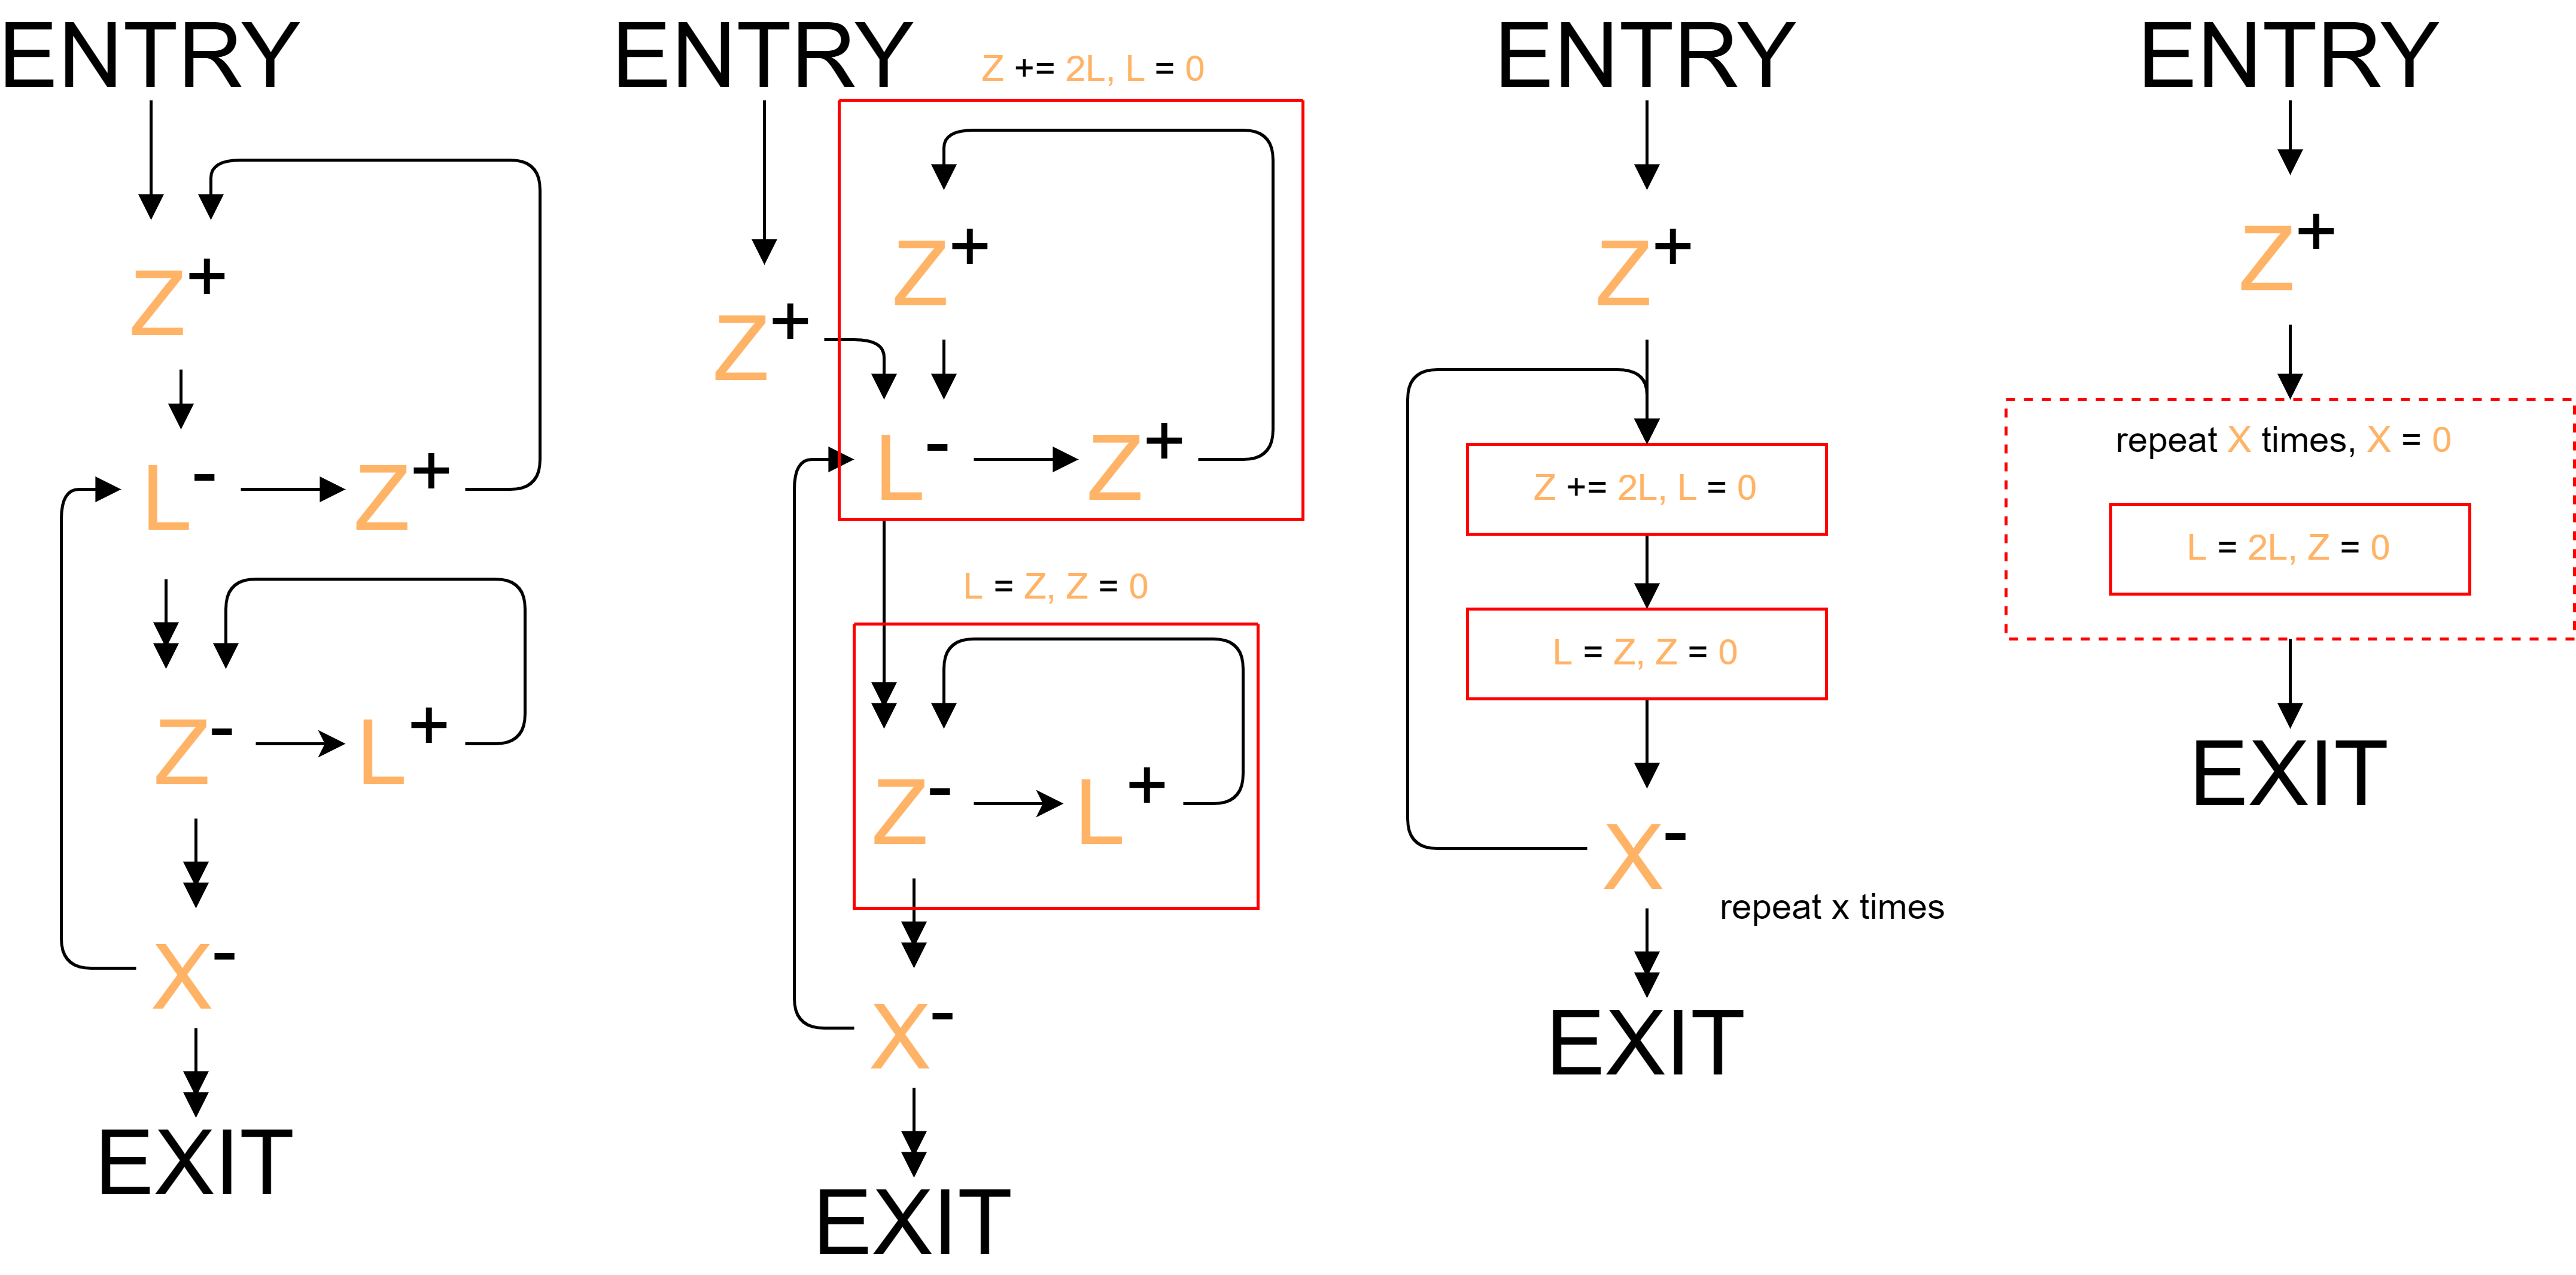
\includegraphics[width=0.9\textwidth]{register_machines/images/rm_analysis.drawio.png}
\end{center}

\subsection{Invariants}
We can use logical assertions on the register machine state at certain instructions, both to get the result of the register machine, and to prove the result.
\\
\\ If correct, every execution path to a given instruction's invariant, establishes that invariant.
\\
\\ We could attach invariants to every instruction, however it is usually only necessary to use them at the start, end and for loops (preconditions/postconditions).
\begin{center}
    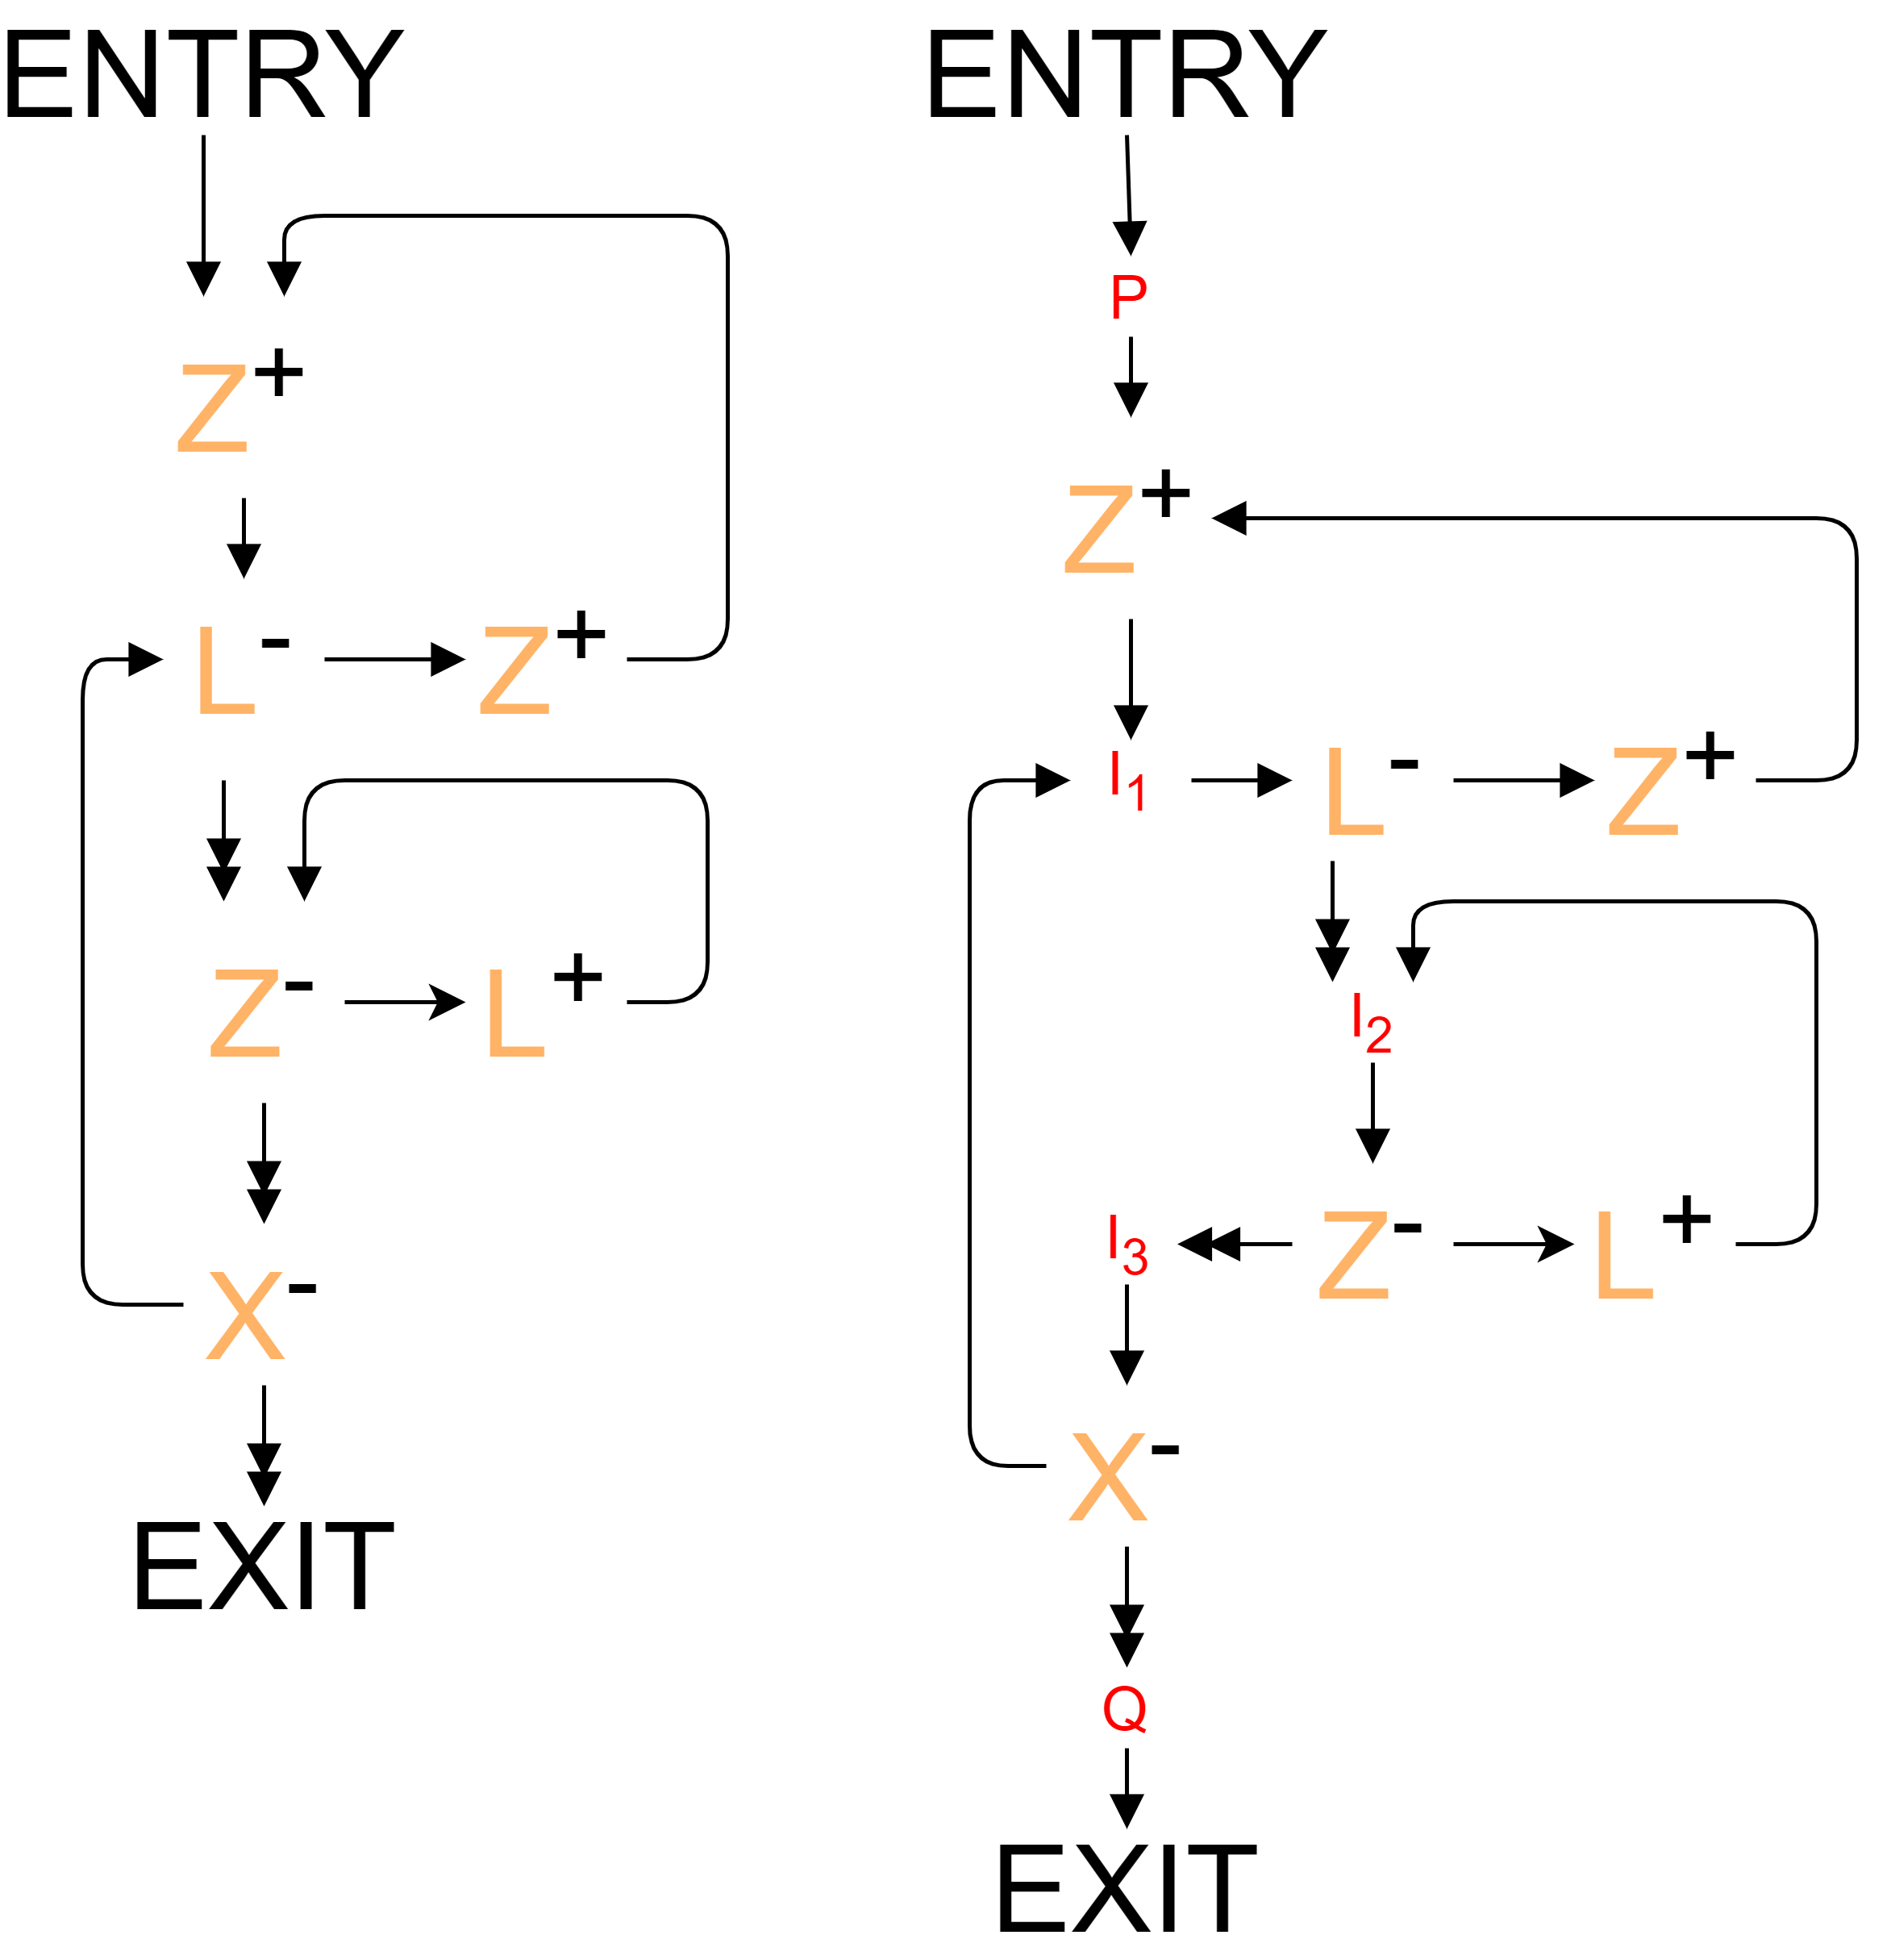
\includegraphics[width=0.4\textwidth]{register_machines/images/rm_analysis_invariants.drawio.png}
\end{center}
Our first invariant ($P$) can be defined as:
\[P \equiv (X =x  \land L = l \land Z = 0)\]
Next we can use the instructions between invariant to find the states under which the invariants must hold.
\begin{center}
    \begin{tabular}{l l p{0.7\textwidth}}
        \textbf{1.} & $P[Z-1/Z] \Rightarrow I_1$              & After incrementing $Z$ needs to go to the start of the first loop.                                  \\
        \hline
        \textbf{2.} & $I_1[L + 1/L, Z - 2/Z] \Rightarrow I_1$ & The loop decrements $L$ and increases $Z$ by two. After each loop iteration, $I_1$ must still hold. \\
        \hline
        \textbf{3.} & $I_1 \land L = 0 \Rightarrow I_2$       & If $L = 0$ the loop is escaped, and we move to $I_2$.                                               \\
        \hline
        \textbf{4.} & $I_2[Z+1/Z,L-1/L] \Rightarrow I_2$      & Loop increments $L$ and decrements $Z$ on each iteration, after this, $I_2$ must still hold.        \\
        \hline
        \textbf{5.} & $I_2 \land Z = 0 \Rightarrow I_3$       & Loop ends when $Z = 0$, moves to $I_3$.                                                             \\
        \hline
        \textbf{6.} & $I_3[X+1/X] \Rightarrow I_1$            & Large loop decrements $X$ on each iteration, invariant must hold with the new/decremented $X$.      \\
        \hline
        \textbf{7.} & $I_3 \land X = 0 \Rightarrow Q$         & When the main $X$-decrementing loop is escaped, we move to exit, so $Q$ must hold.
    \end{tabular}
\end{center}
We can now use these constraints (also called \textit{verification conditions}) to determine an invariant.
\\
\\
\\ For each constraint we do:
\begin{enumerate}
    \item Get the basic for (potentially one already derived) for the invariant in question.
    \item If there is iteration, iterate to build up a disjunction.
    \item Find the pattern, and then re-form the invariant based on it.
\end{enumerate}

\subsubsection*{Constraint 1.}
Hence we can deduce $I_1$ as:
\[I_1 = (X = x \land L = l \land Z = 1)\]
(Take $P$ and increment $Z$)
\subsubsection*{Constraint 2.}
We can iterate to get the disjunction:
\[I_1 \equiv (X=x \land L=l \land Z = 1) \lor (X=x \land L+1 = l \land Z-2 = 1) \lor (X=x \land L+2 = l \land Z - 4 = 1) \lor \dots\]
Hence we can determine the pattern for each disjunct as:
\[Z + 2L = 2l + 1\]
Hence we create our invariant:
\[I_1 = (X = x \land Z + 2L = 2l + 1)\]
\subsubsection*{Constraint 3.}
Hence as $L=0$ we can determine that $Z = 2l + 1$.
\[I_2 = (X=x \land Z = 2l + 1 \land L = 0)\]
\subsubsection*{Constraint 4.}
We iterate to get the disjunction:
\[I_2 = (X = x  \land Z = 2l + 1 \land L = 0) \lor (X = x  \land Z = 2l + 0 \land L = 1) \lor (X = x  \land Z = 2l - 1 \land L = 2) \lor \dots\]
Hence we notice the pattern:
\[Z + L = 2l + 1\]
So can deduce the invariant:
\[I_2 = (X = x \land Z + L = 2l + 1)\]
\subsubsection*{Constraint 5.}
We can derive an invariant $I_3$ using $Z = 0$.
\[I_3 = (X=x \land L = 2l + 1 \land Z = 0)\]
\subsubsection*{Constraint 6.}
We can use the constraint, and the currently derived $I_1$ to get a disjunction:
\[I_1 = (X=x-1 \land L = 2l + 1 \land Z = 0) \lor (X = x \land Z + 2L = 2l + 1)\]
We can apply constraint \textbf{2.} on the first part of this disjunction, iterating to get the disjunction:
\[I_1 = (X = x \land Z + 2L = 2l + 1) \lor \left( \begin{matrix}
            (X=x-1 \land L = 2l + 1 \land Z = 0) \lor     \\
            (X=x-1 \land L = 2l + 0 \land Z = 2) \lor     \\
            (X=x-1 \land L = 2l-1 \land Z = 4) \lor       \\
            (X=x-1 \land L = 2l-2 \land Z = 8) \lor \dots \\
        \end{matrix} \right)\]
Hence for the second group of disjuncts we have the relation:
\[Z + 2L = 2(2l + 1)\]
Hence we have:
\[I_1 = (X = x \land Z + 2L = 2l + 1) \lor (X=x-1 \land Z + 2L = 2(2l + 1))\]
Hence when we repeat on the larger loop, we will double again, iterating we get:
\[I_1 = (X = x \land Z + 2L = 2l + 1) \lor (X=x-1 \land Z + 2L = 2(2l + 1)) \lor (X=x-2 \land Z + 2L = 4(2l + 1)) \lor \dots\]
Hence we have the relation:
\[I_1 = (Z + 2L = 2^{X - x}(2l + 1))\]
We can apply this doubling to $L_2$ also as it forms part of the larger loop:
\[I_2 = (Z + L = 2^{X - x}(2l + 1))\]
And to $I_3$:
\[I_3 = (L = 2^{X-x}(2l + 1) \land Z = 0)\]

\subsubsection*{Constraint 7.}
Hence we can now derive $Q$ as:
\[Q = (L = 2^x(2l + 1) \land Z = 0)\]

\subsubsection*{Termination}
We also need to show that each of our loops eventually terminate, we can do this by showing that sme variant (e.g register, or combination of) decreases every time the invariant is reached/visited.
\\
\\ For $I_1$ we can use the lexicographical ordering $(X,L)$ as in each inner loop $L$ decreases, but for the larger loop while $L$ is reset/does not increase, $X$ does.
\\
\\ For $I_2$ we can similarly use the lexicographical ordering $(X,Z)$
\\
\\ For $I_3$ we can just use $X$.


\section{Universal Register Machine}
A register machine that simulates a register machine.
\\
\\ It takes the arguments:
\begin{center}
    \begin{tabular}{l p{.7\textwidth}}
        $\reglabel{0}$ & $= 0$ \\
        $\reglabel{1}$ & $= $ the program encoded as a number \\
        $\reglabel{2}$ & $= $ the argument list encoded as a number \\
        \multicolumn{2}{c}{All other registers zeroed} \\
    \end{tabular}
\end{center}
The registers used are:
\begin{center}
	\begin{tabular}{l l p{0.7\textwidth}}
		$\reglabel{1}$      & P  & Program code of the register machine being simulated/emulated.                              \\
		$\reglabel{2}$      & A  & Arguments provided to the simulated register machine.                                       \\
		$\reglabel{3}$      & PC & Program Counter - The current register machine instruction.                                 \\
		$\reglabel{4}$      & N  & Next label num,ber/next instruction to go to. Is also used to store the current instruction \\
		$\reglabel{5}$      & C  & The current instruction.                                                                    \\
		$\reglabel{6}$      & R  & The value of the register used by the current instruction.                                  \\
		$\reglabel{7}$      & S  & Auxiliary Register                                                                          \\
		$\reglabel{8}$      & T  & Auxiliary Register                                                                          \\
		$\reglabel{9}\dots$ &    & Scratch Registers                                                                           \\
	\end{tabular}
\end{center}
\inputminted{python}{register_machines/code/universal_register_machine.py}
\begin{center}
    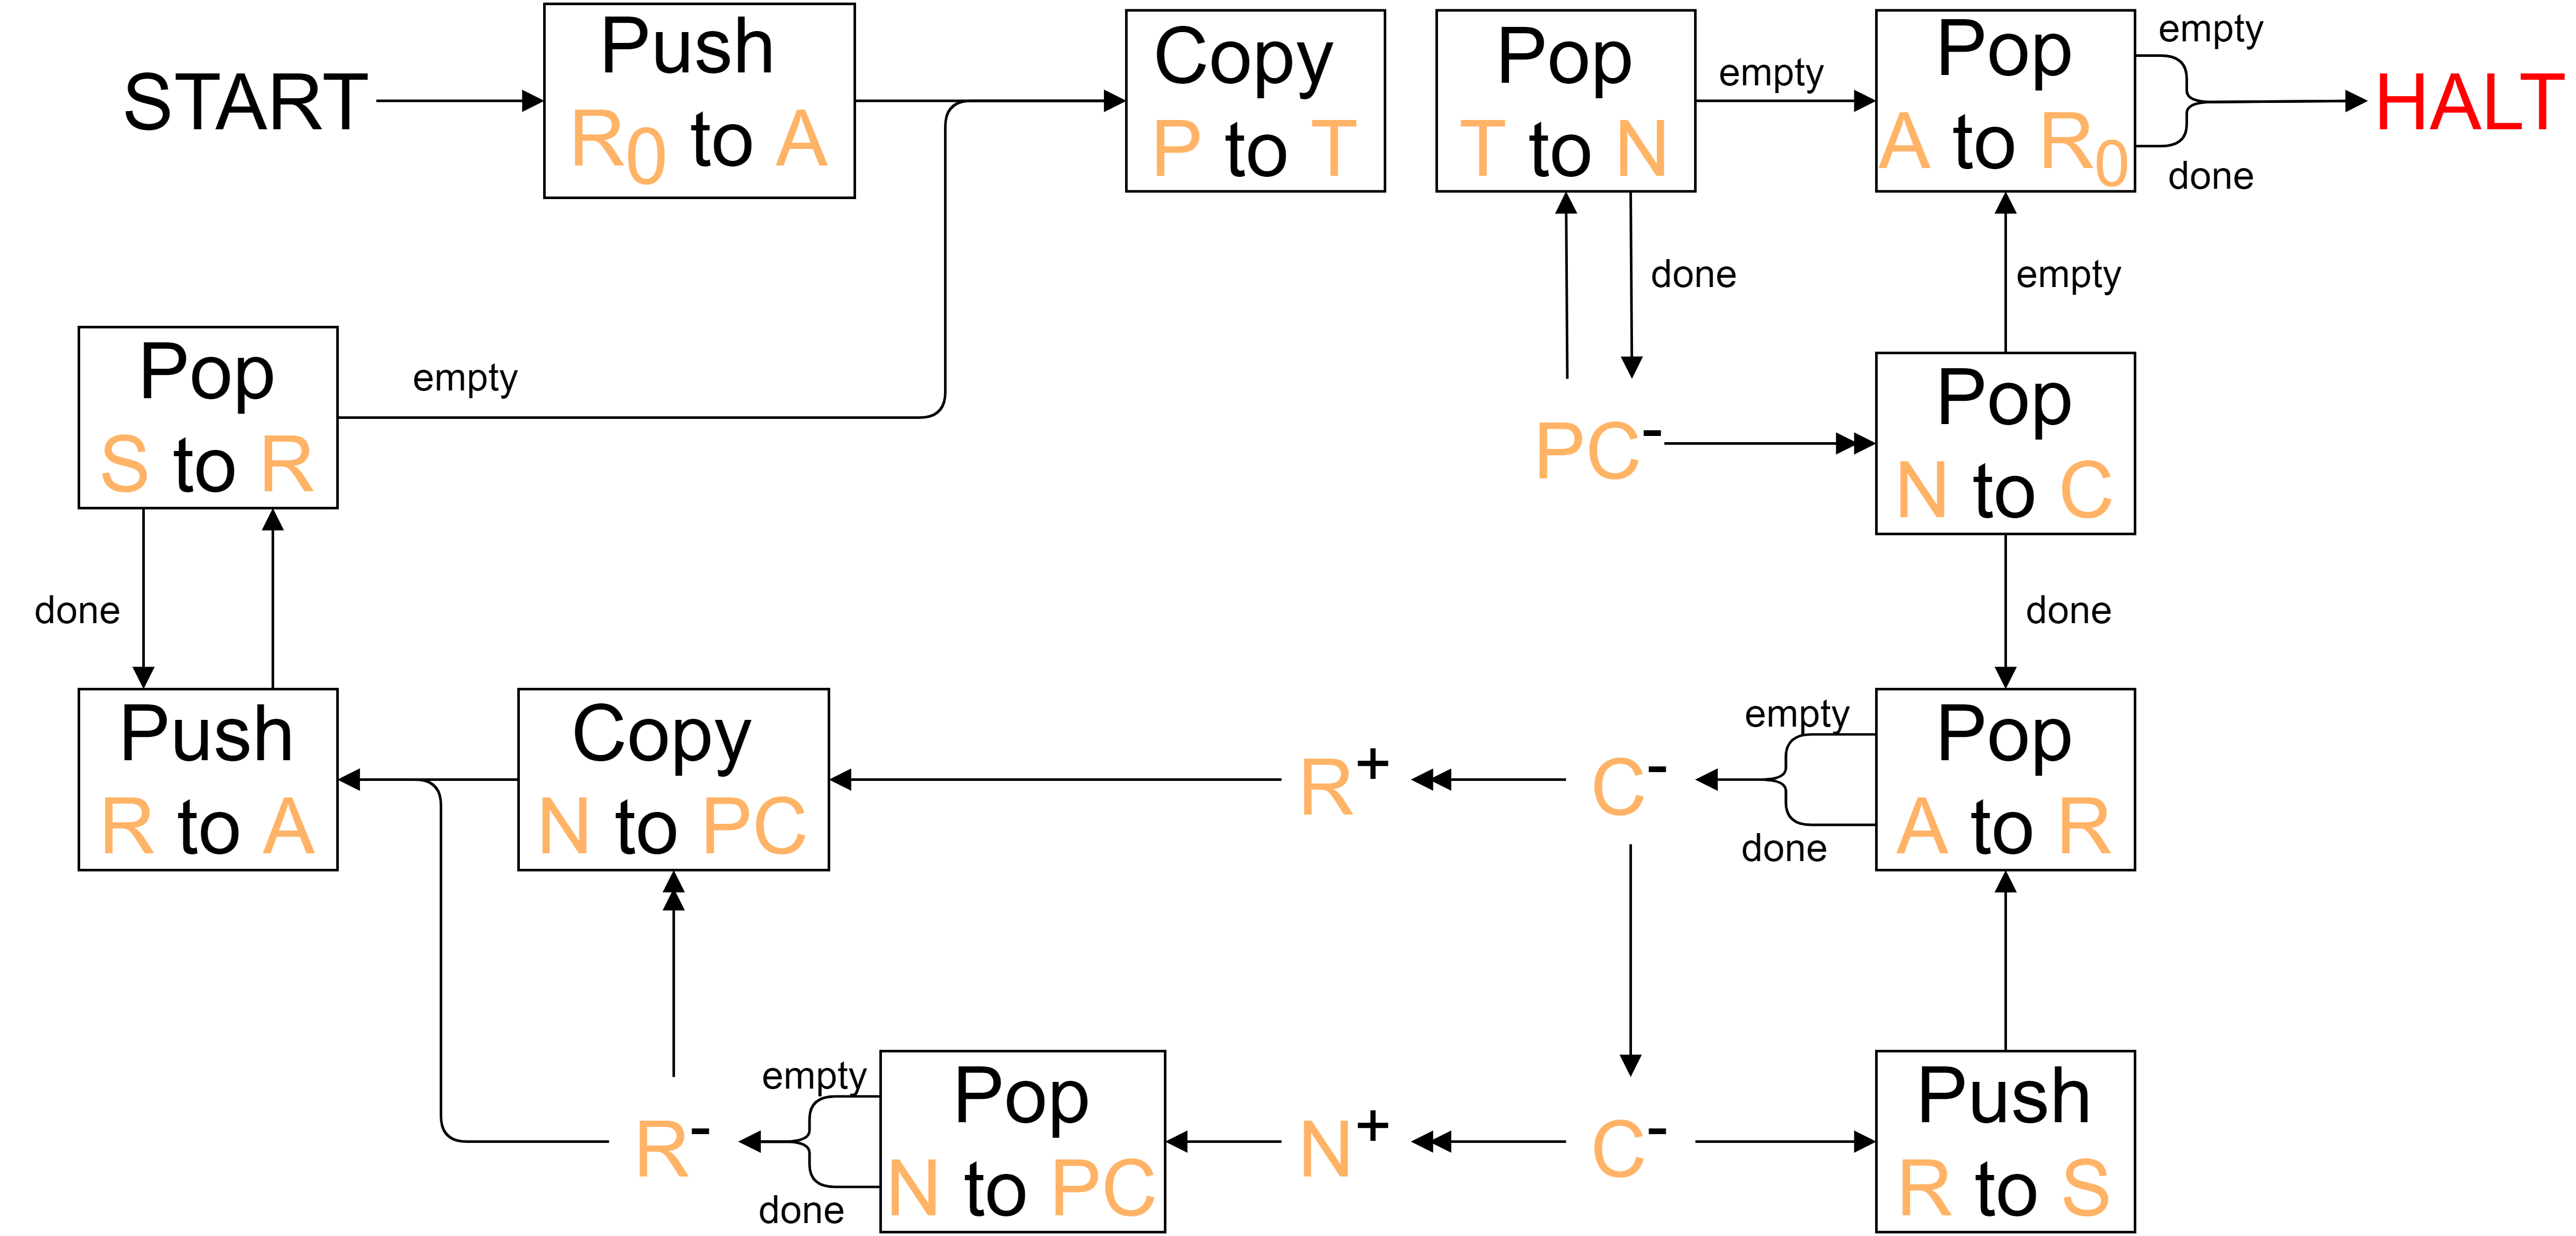
\includegraphics[width=0.9\textwidth]{register_machines/images/universal_register_machine.drawio.png}
\end{center}
